% Content below is autogenerated 
\subsection{Technical details on low-power jammer 'S1.1'}
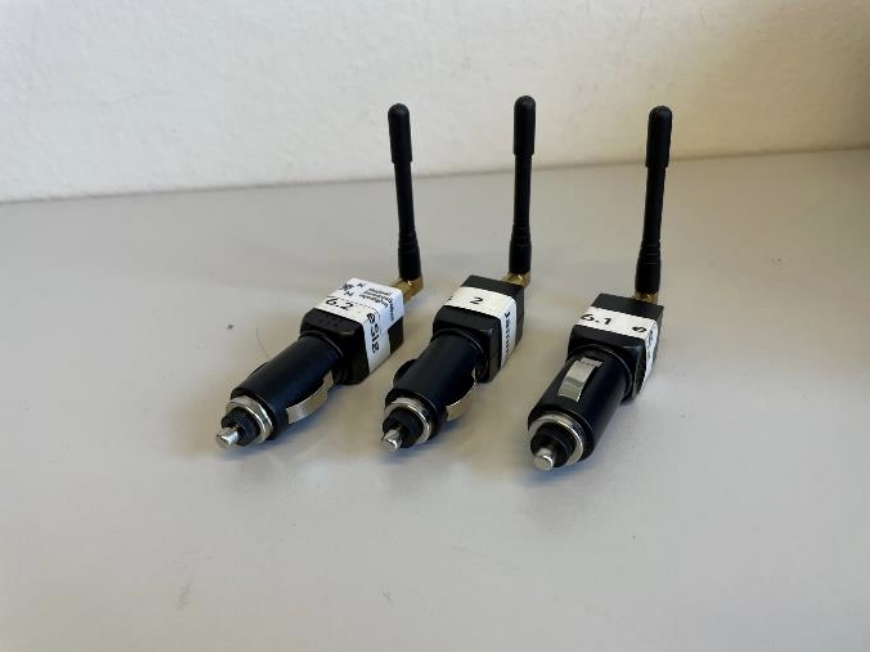
\includegraphics[scale=0.4]{../graphics/appendixG/s1.1-photo.png}\\ \\ 
The jammer S1.1 belongs to the 'Cigarette jammer' category of jammers. Such jammers are often installed in the cigarette lighter outlet in cars. They are intended to cover the car, and a given radius around the car. \\S1.1 is an one-antenna, so-called 'L1-only', jammer, disrupting only the upper L-band.\\
\begin{table}[H]\centering
\begin{tabular}{|c|c|c|c|c|c|c|}\rowcolor[HTML]{C0C0C0} 
\hline
\makecell{Centre frequency\\{[MHz]}} & \makecell{Bandwidth\\{[MHz]}} & \makecell{PSD\\{[dBm/MHz]}} & \makecell{TX total\\{[dBm]}} & \makecell{CF max\\{[dBm]}} & \makecell{Sweep rate\\{[µs]}} & \makecell{Modulation}\\ 
\hline
\makecell{1577.40} & \makecell{29.96} & \makecell{7.58} & \makecell{22.34} & \makecell{7.89} & \makecell{37.1} & \makecell{Sawtooth}\\ 
\hline\end{tabular}\caption{Technical characteristics of S1.1 jammer}\label{table:tech_char_S1.1}\end{table}
\begin{figure}[H]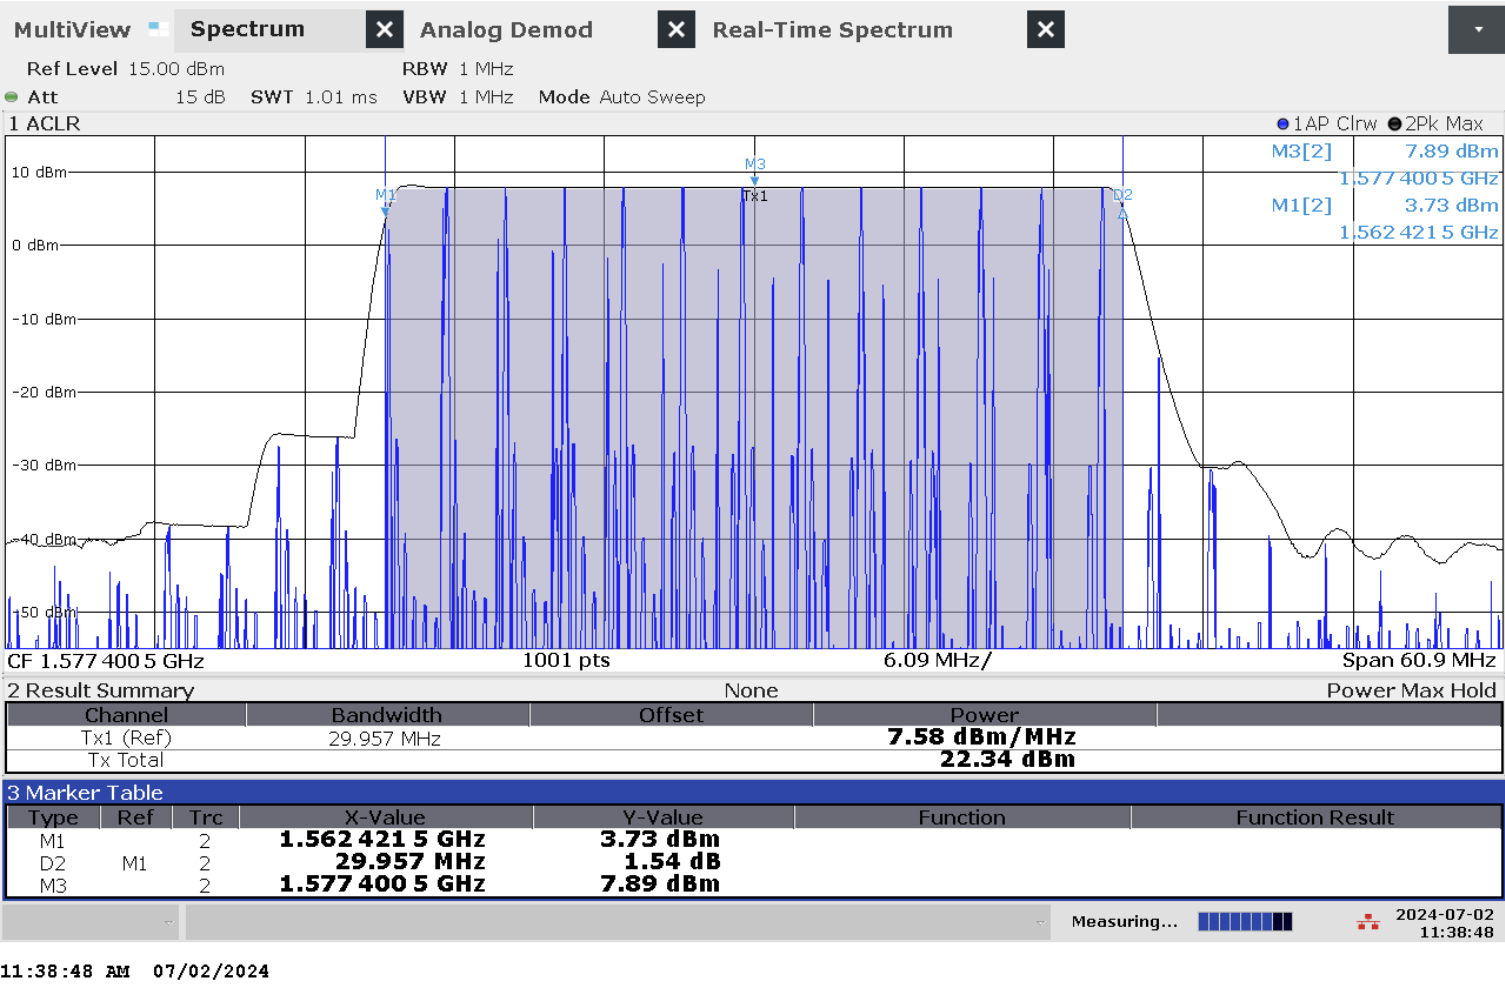
\includegraphics[width=\textwidth]{../graphics/appendixG/s1.1-1.png} 
\caption{Frequency and power measurement of jammer S1.1}\end{figure}\begin{figure}[H]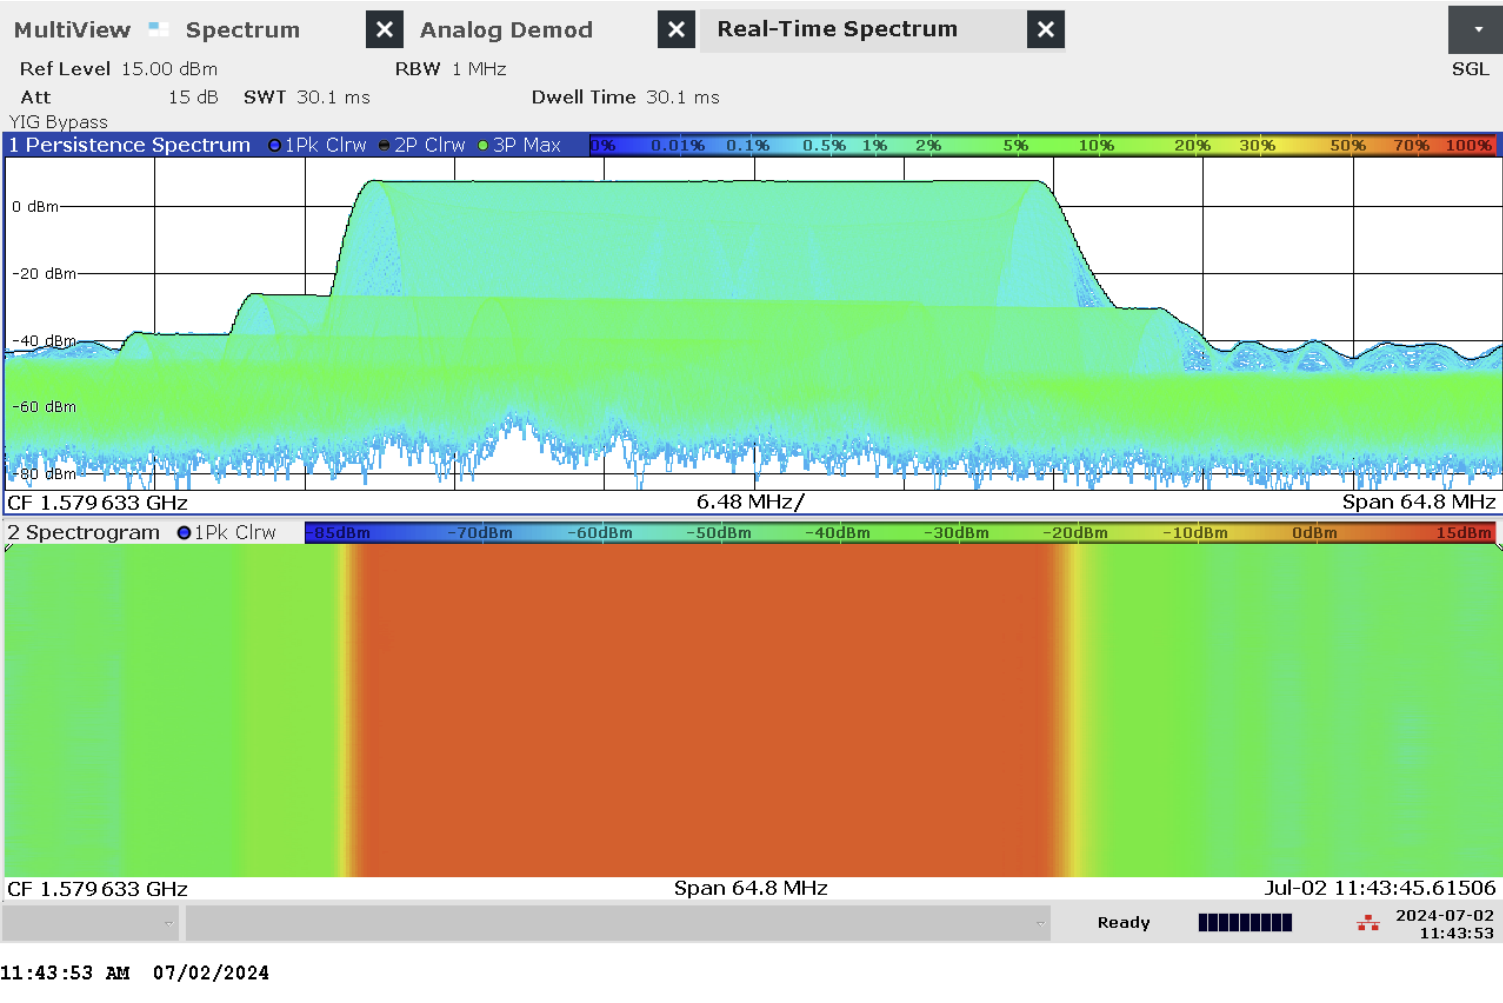
\includegraphics[width=\textwidth]{../graphics/appendixG/s1.1-2.png} 
\caption{Real-time persistence and spectrogram measurement of jammer S1.1}\end{figure}\begin{figure}[H]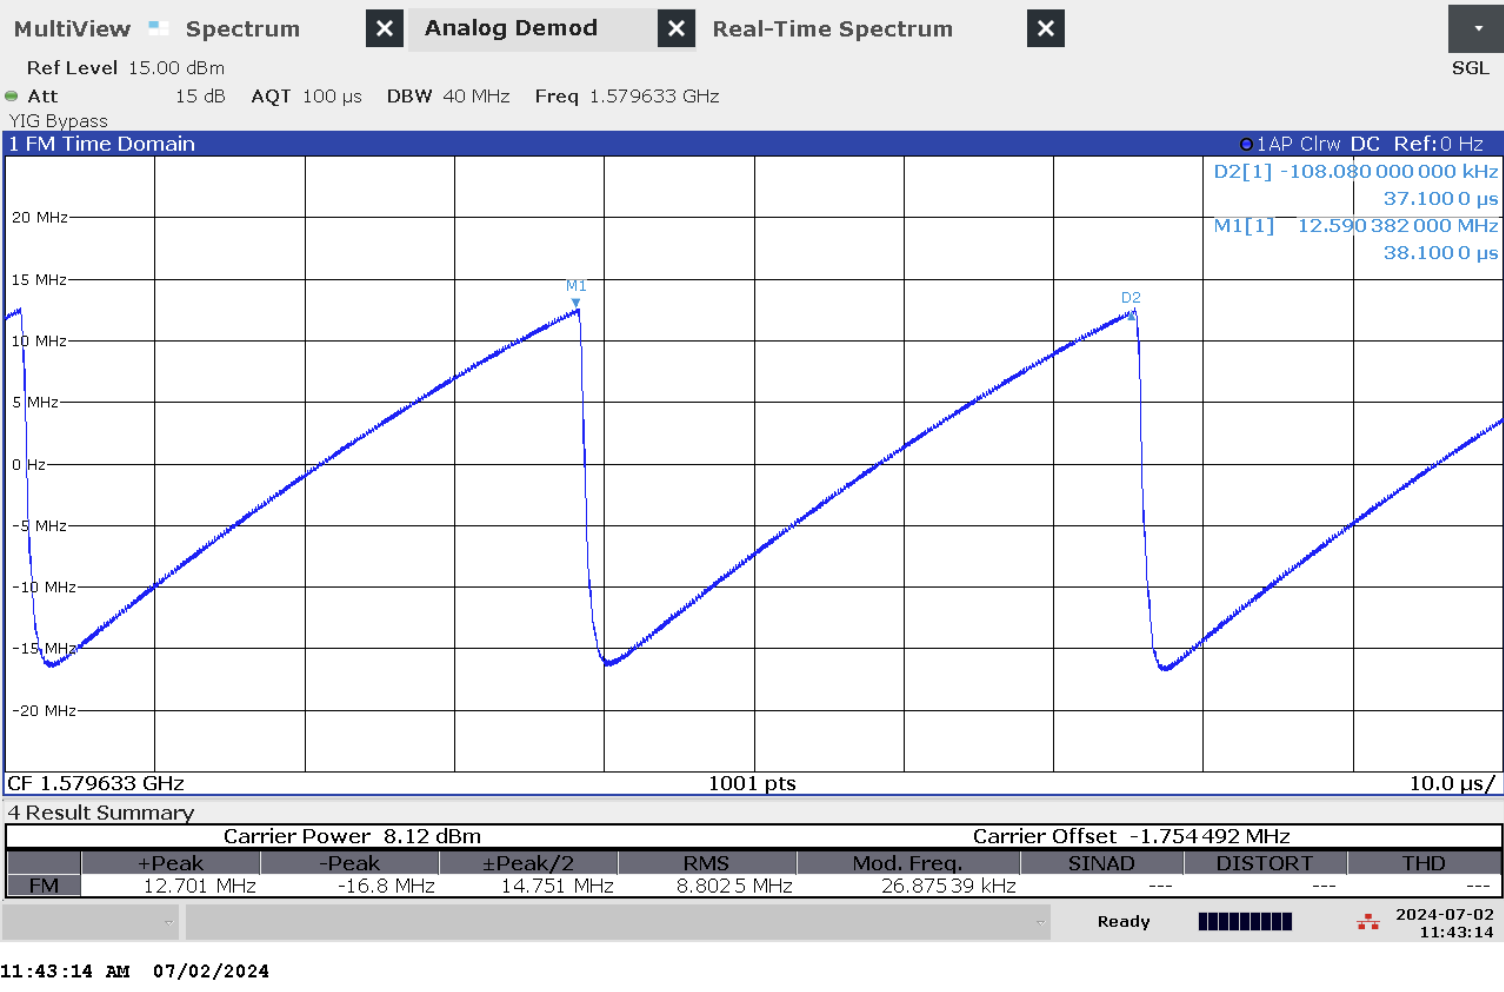
\includegraphics[width=\textwidth]{../graphics/appendixG/s1.1-3.png} 
\caption{Time domain (analog demod) measurement of jammer S1.1}\end{figure}\subsection{Technical details on low-power jammer 'S1.2'}
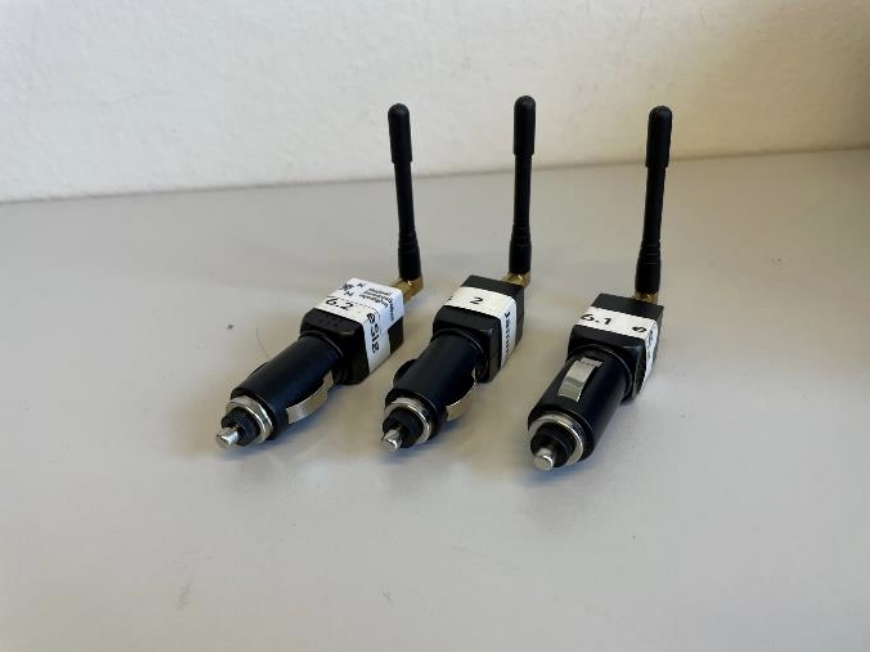
\includegraphics[scale=0.4]{../graphics/appendixG/s1.1-photo.png}\\ \\ 
The jammer S1.2 belongs to the 'Cigarette jammer' category of jammers. Such jammers are often installed in the cigarette lighter outlet in cars. They are intended to cover the car, and a given radius around the car. \\S1.2 is an one-antenna, so-called 'L1-only', jammer, disrupting only the upper L-band.\\
\begin{table}[H]\centering
\begin{tabular}{|c|c|c|c|c|c|c|}\rowcolor[HTML]{C0C0C0} 
\hline
\makecell{Centre frequency\\{[MHz]}} & \makecell{Bandwidth\\{[MHz]}} & \makecell{PSD\\{[dBm/MHz]}} & \makecell{TX total\\{[dBm]}} & \makecell{CF max\\{[dBm]}} & \makecell{Sweep rate\\{[µs]}} & \makecell{Modulation}\\ 
\hline
\makecell{1582.56} & \makecell{40.03} & \makecell{12.38} & \makecell{29.01} & \makecell{12.61} & \makecell{21.56} & \makecell{Sawtooth}\\ 
\hline\end{tabular}\caption{Technical characteristics of S1.2 jammer}\label{table:tech_char_S1.2}\end{table}
\begin{figure}[H]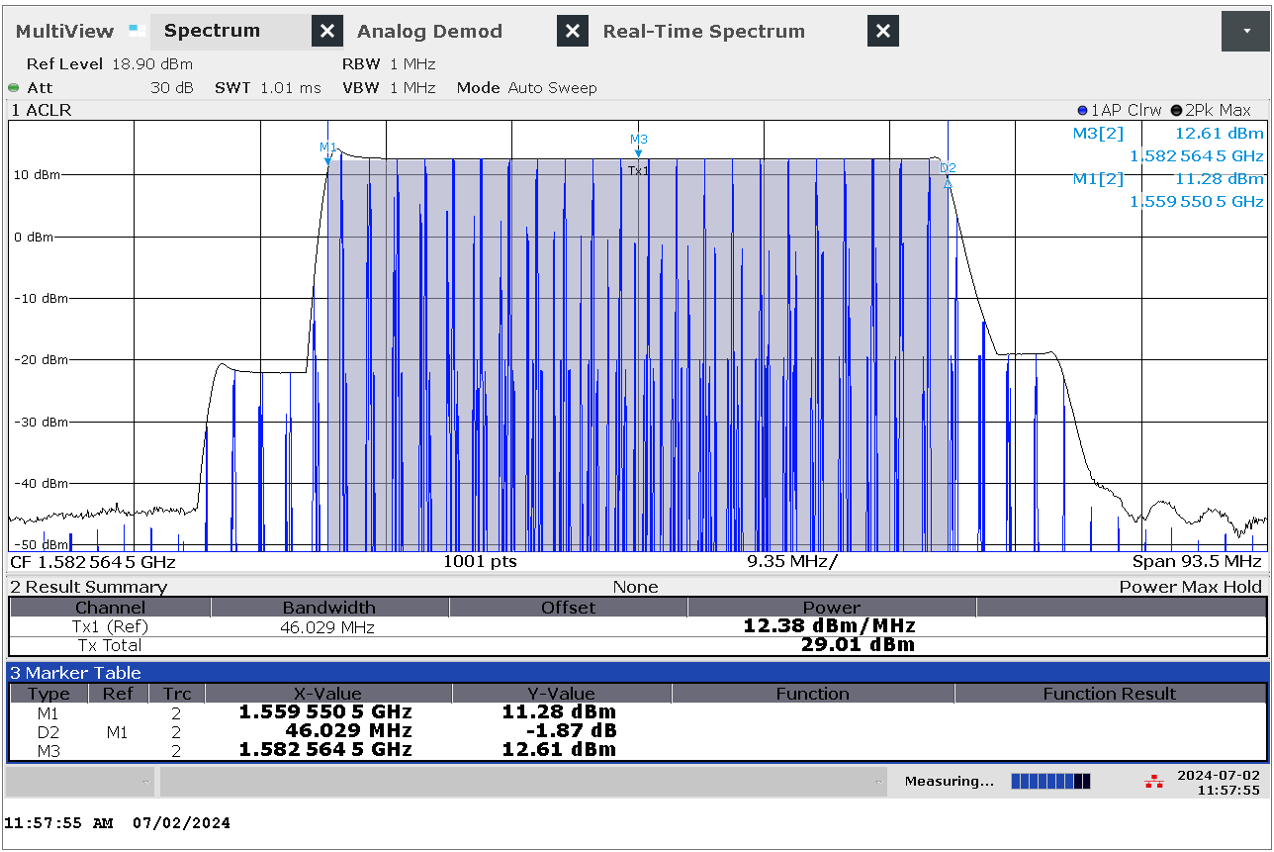
\includegraphics[width=\textwidth]{../graphics/appendixG/s1.2-1.png} 
\caption{Frequency and power measurement of jammer S1.2}\end{figure}\begin{figure}[H]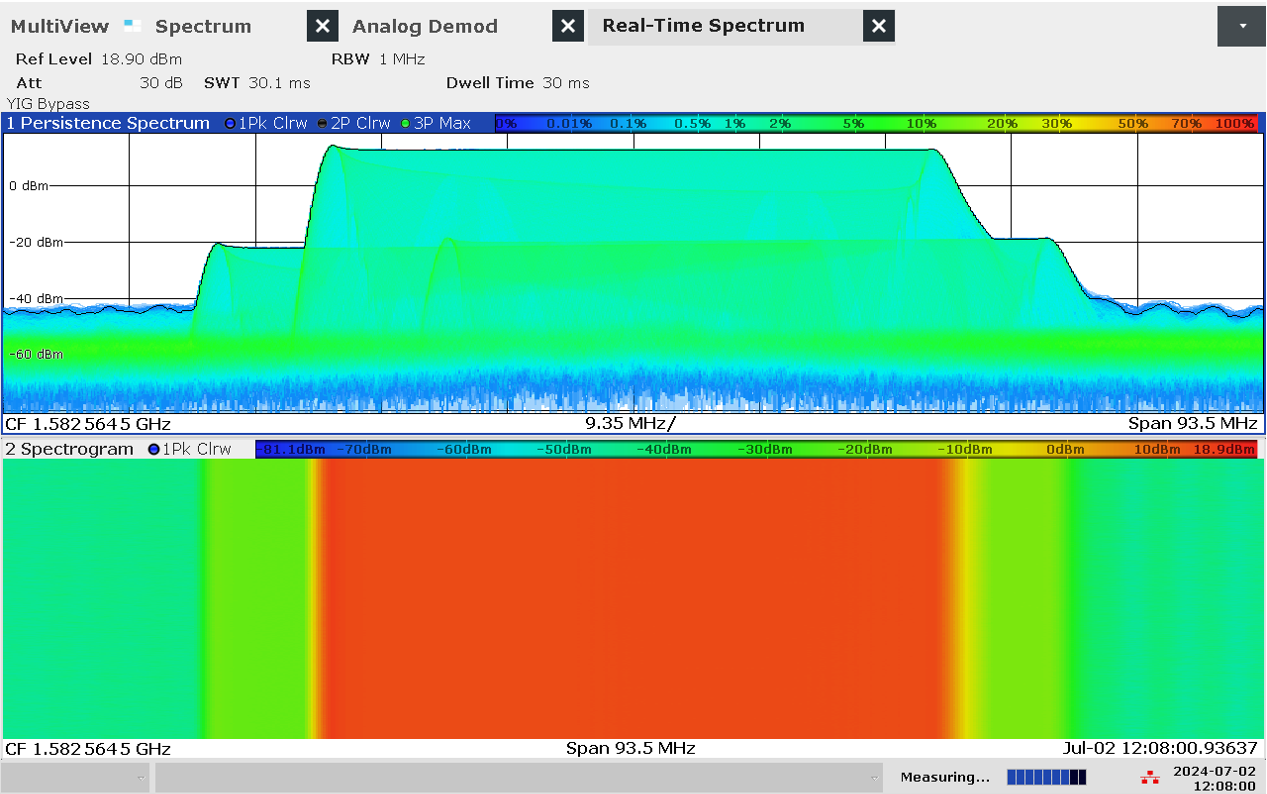
\includegraphics[width=\textwidth]{../graphics/appendixG/s1.2-2.png} 
\caption{Real-time persistence and spectrogram measurement of jammer S1.2}\end{figure}\begin{figure}[H]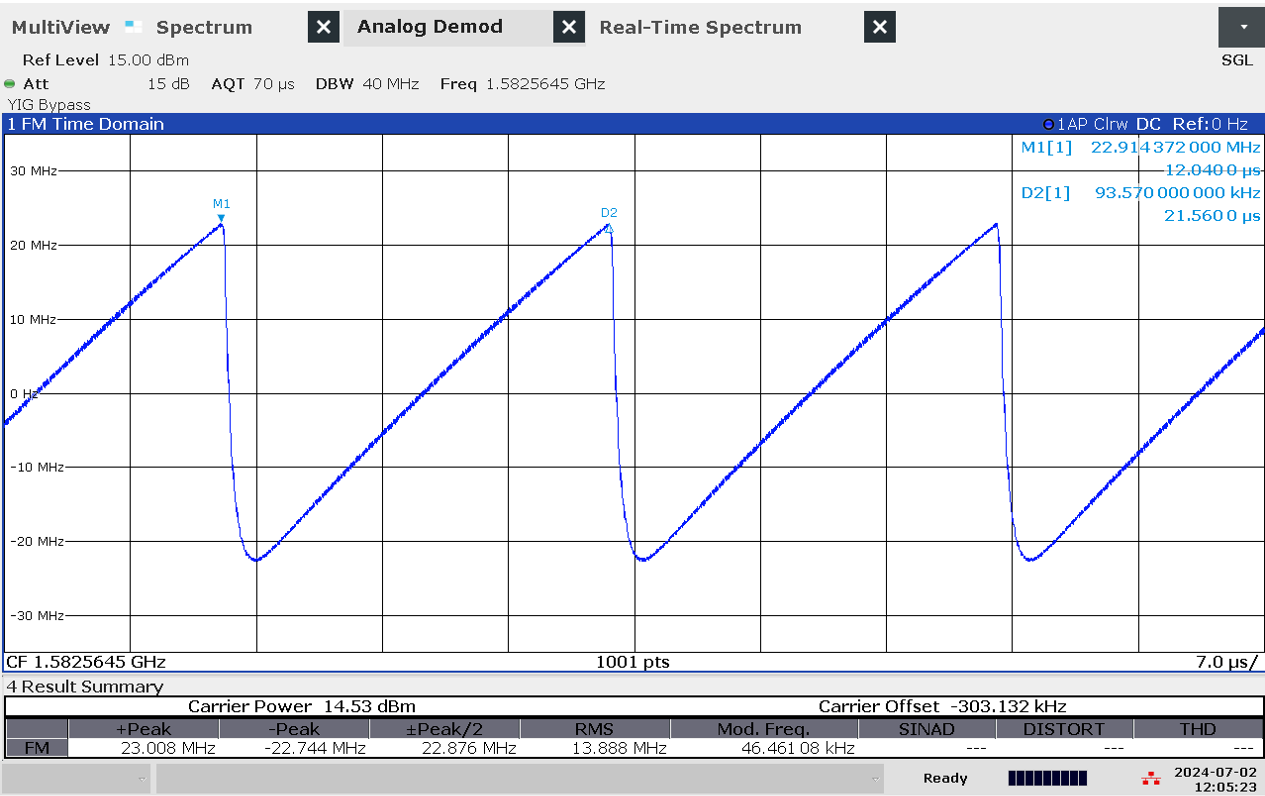
\includegraphics[width=\textwidth]{../graphics/appendixG/s1.2-3.png} 
\caption{Time domain (analog demod) measurement of jammer S1.2}\end{figure}\subsection{Technical details on low-power jammer 'S1.3'}
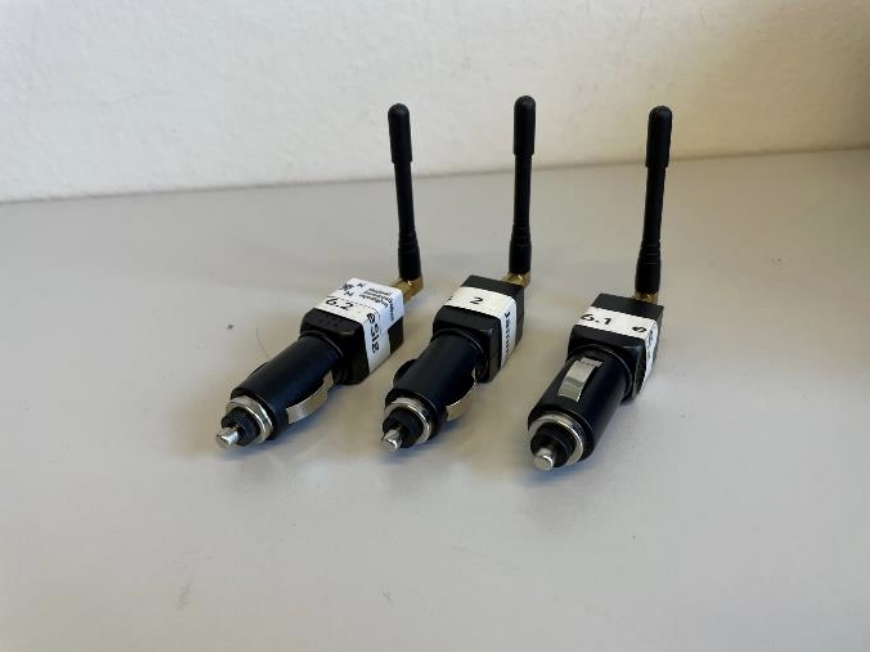
\includegraphics[scale=0.4]{../graphics/appendixG/s1.1-photo.png}\\ \\ 
The jammer S1.3 belongs to the 'Cigarette jammer' category of jammers. Such jammers are often installed in the cigarette lighter outlet in cars. They are intended to cover the car, and a given radius around the car. \\S1.3 is an one-antenna, so-called 'L1-only', jammer, disrupting only the upper L-band.\\
\begin{table}[H]\centering
\begin{tabular}{|c|c|c|c|c|c|c|}\rowcolor[HTML]{C0C0C0} 
\hline
\makecell{Centre frequency\\{[MHz]}} & \makecell{Bandwidth\\{[MHz]}} & \makecell{PSD\\{[dBm/MHz]}} & \makecell{TX total\\{[dBm]}} & \makecell{CF max\\{[dBm]}} & \makecell{Sweep rate\\{[µs]}} & \makecell{Modulation}\\ 
\hline
\makecell{1579.63} & \makecell{31.88} & \makecell{7.56} & \makecell{22.60} & \makecell{7.93} & \makecell{37.5} & \makecell{Sawtooth}\\ 
\hline\end{tabular}\caption{Technical characteristics of S1.3 jammer}\label{table:tech_char_S1.3}\end{table}
\begin{figure}[H]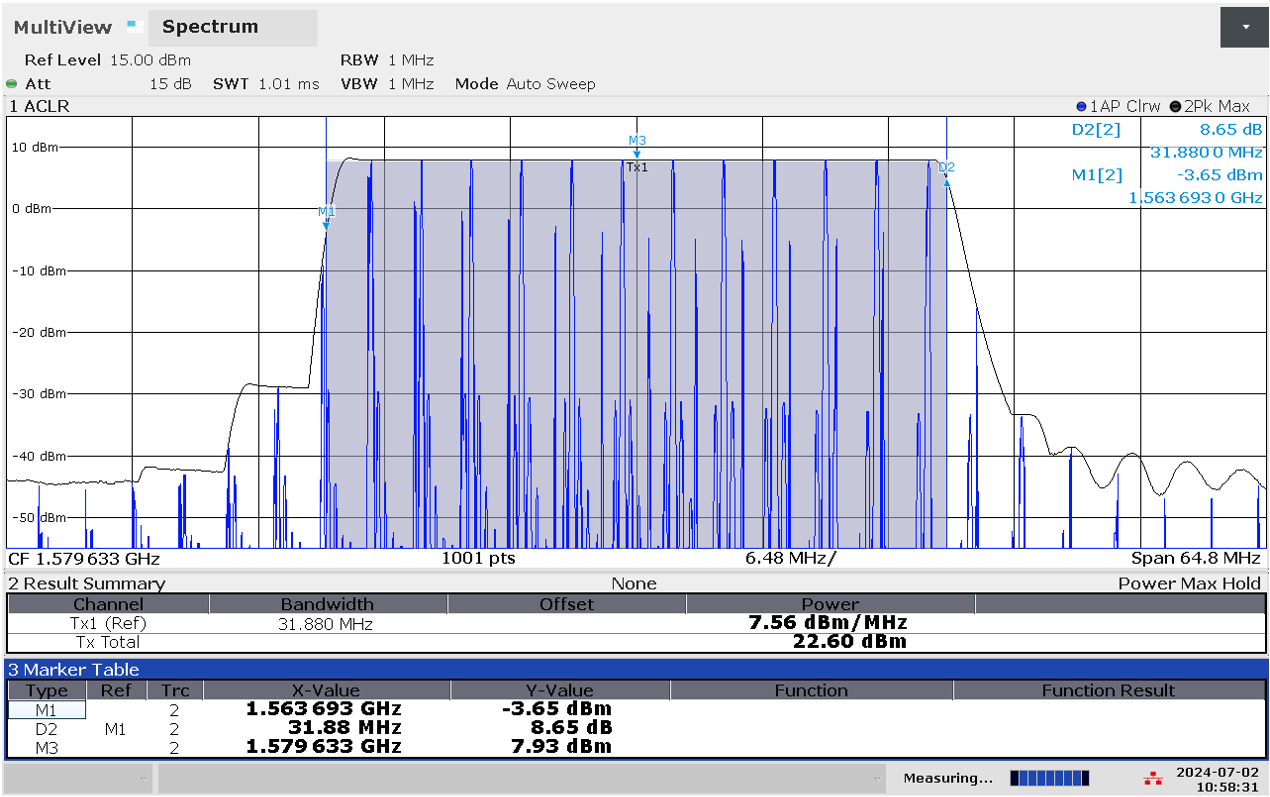
\includegraphics[width=\textwidth]{../graphics/appendixG/s1.3-1.png} 
\caption{Frequency and power measurement of jammer S1.3}\end{figure}\begin{figure}[H]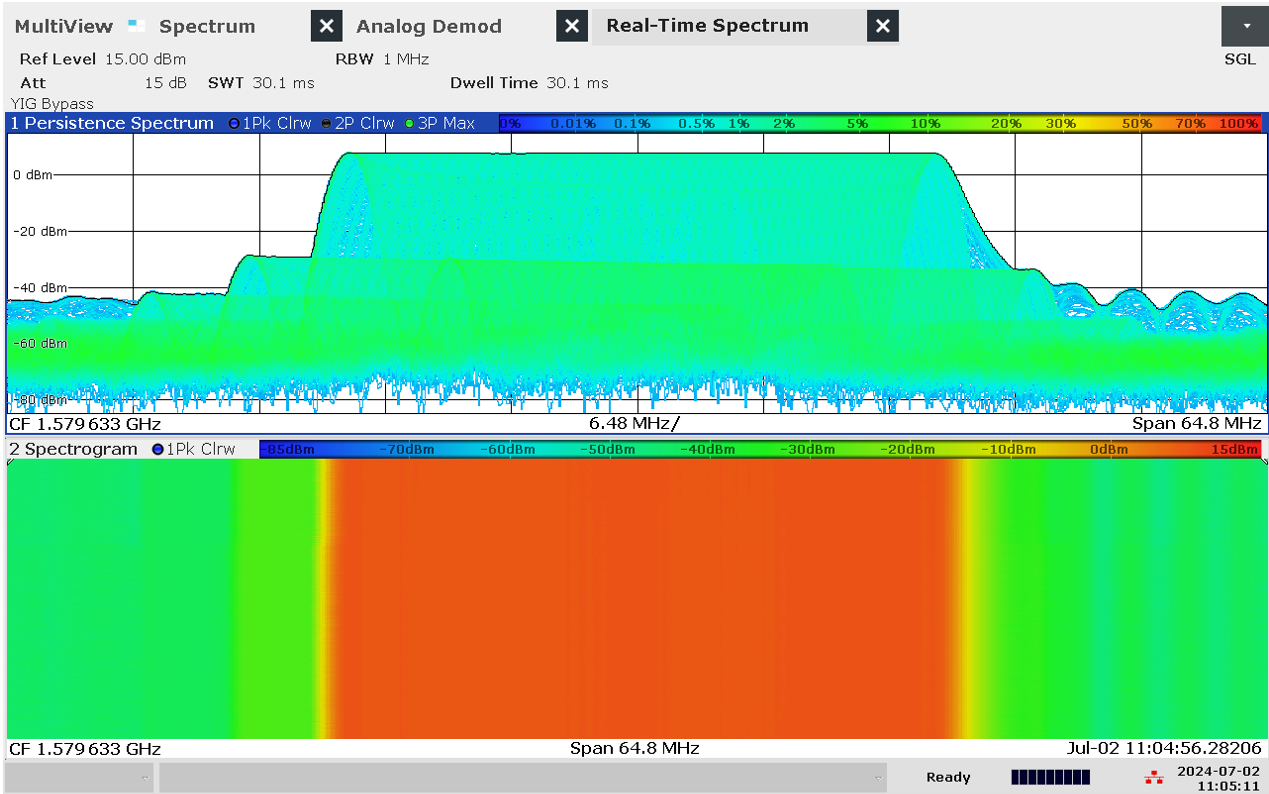
\includegraphics[width=\textwidth]{../graphics/appendixG/s1.3-2.png} 
\caption{Real-time persistence and spectrogram measurement of jammer S1.3}\end{figure}\begin{figure}[H]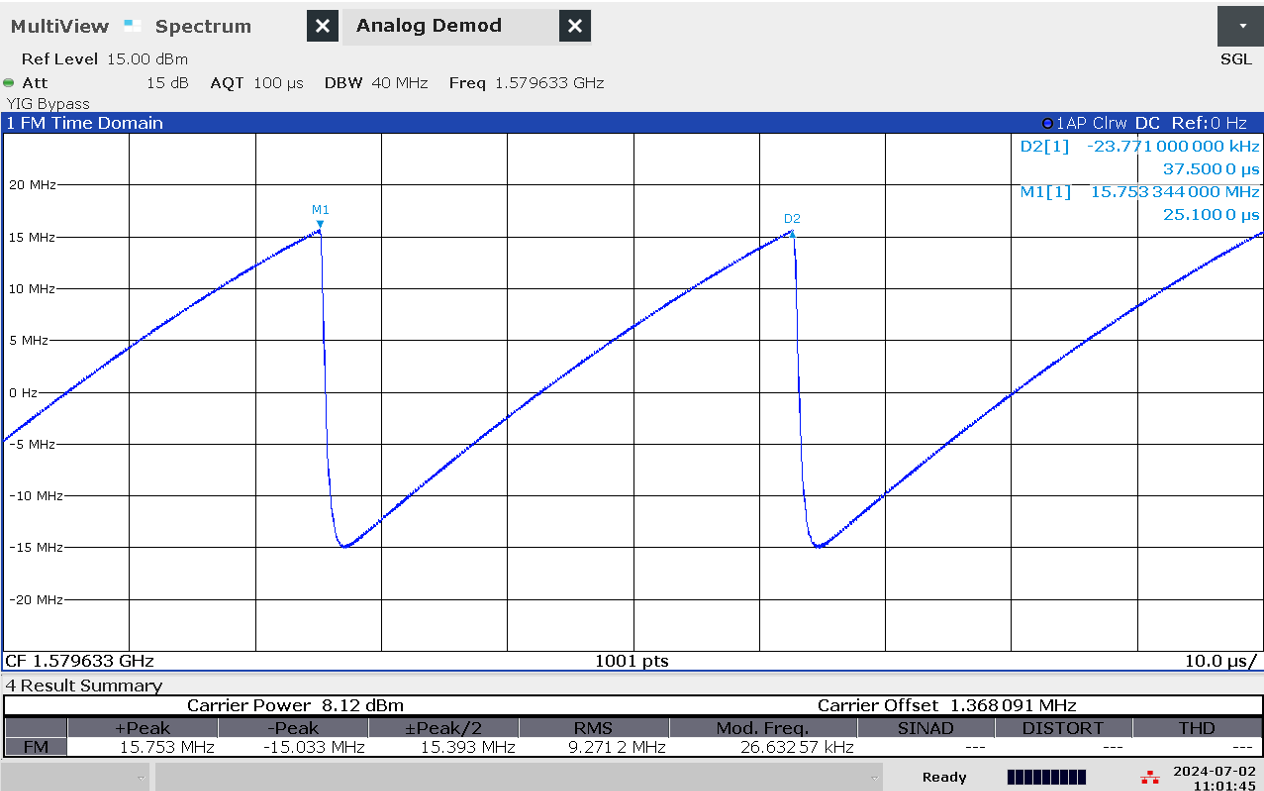
\includegraphics[width=\textwidth]{../graphics/appendixG/s1.3-3.png} 
\caption{Time domain (analog demod) measurement of jammer S1.3}\end{figure}\subsection{Technical details on low-power jammer 'S2.1'}
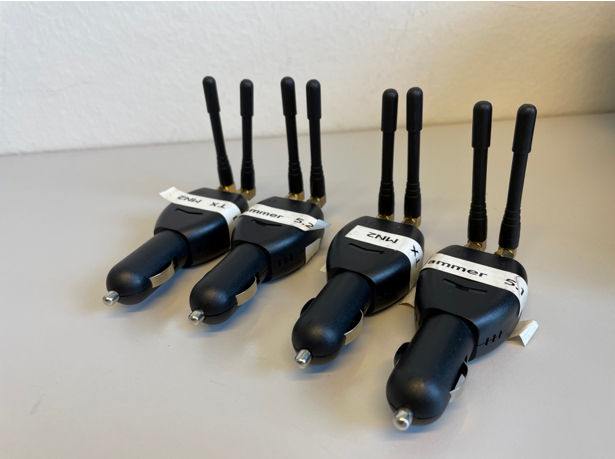
\includegraphics[scale=0.4]{../graphics/appendixG/s2.1-photo.png}\\ \\ 
The jammer S2.1 belongs to the 'Cigarette jammer' category of jammers. Such jammers are often installed in the cigarette lighter outlet in cars. They are intended to cover the car, and a given radius around the car. \\S2.1 is a two-antenna, so-called 'L1+L2', jammer, disrupting both the upper and lower L-band.\\
\begin{table}[H]\centering
\begin{tabular}{|c|c|c|c|c|c|c|c|}\rowcolor[HTML]{C0C0C0} 
\hline
\makecell{Antenna} & \makecell{Centre frequency\\{[MHz]}} & \makecell{Bandwidth\\{[MHz]}} & \makecell{PSD\\{[dBm/MHz]}} & \makecell{TX total\\{[dBm]}} & \makecell{CF max\\{[dBm]}} & \makecell{Sweep rate\\{[µs]}} & \makecell{Modulation}\\ 
\hline
\makecell{L1} & \makecell{1581.59} & \makecell{85.41} & \makecell{13.36} & \makecell{32.68} & \makecell{16.64} & \makecell{40.63} & \makecell{Sawtooth+burst}\\ 
\hline
\makecell{L2} & \makecell{1198.05} & \makecell{96.58} & \makecell{13.92} & \makecell{33.75} & \makecell{17.30} & \makecell{42.1} & \makecell{Sawtooth+burst}\\ 
\hline\end{tabular}\caption{Technical characteristics of S2.1 jammer}\label{table:tech_char_S2.1}\end{table}
\begin{figure}[H]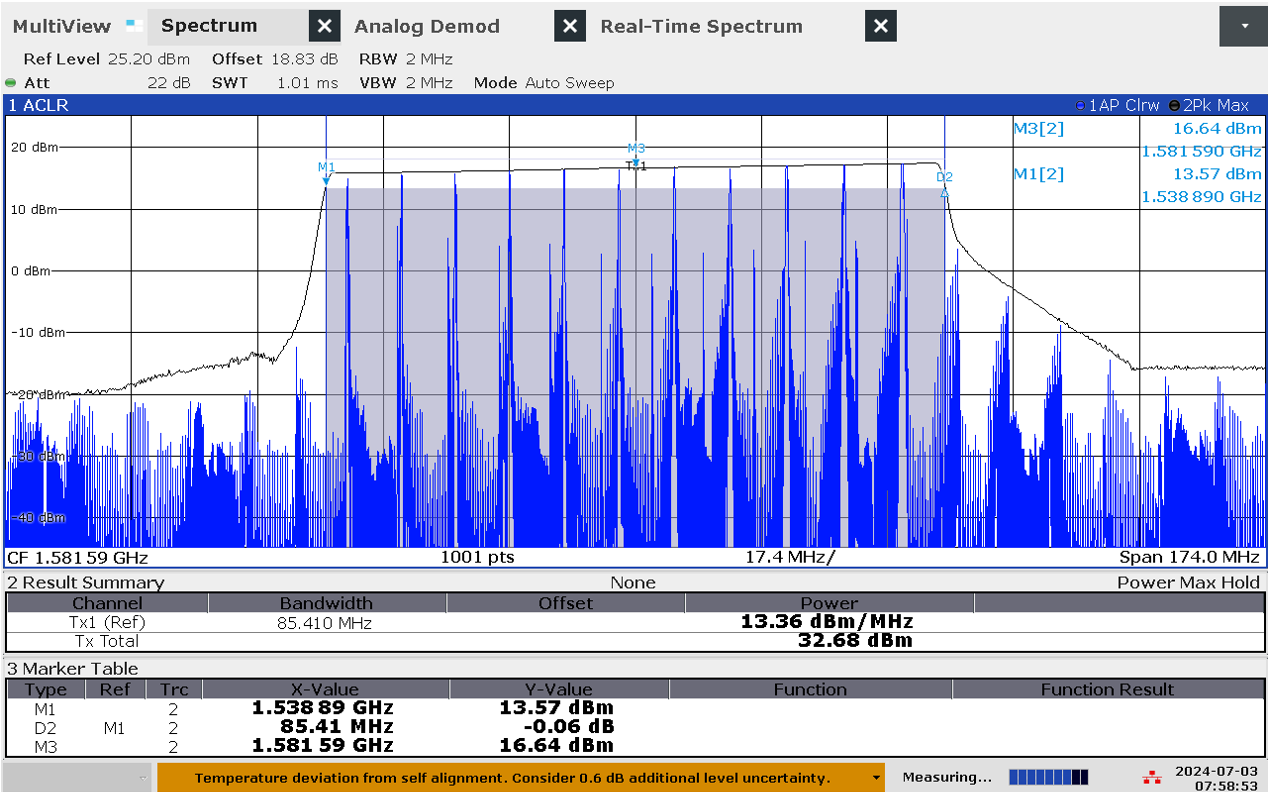
\includegraphics[width=\textwidth]{../graphics/appendixG/s2.1-1.png} 
\caption{Frequency and power measurement of jammer S2.1 on antenna 'L1'}\end{figure}\begin{figure}[H]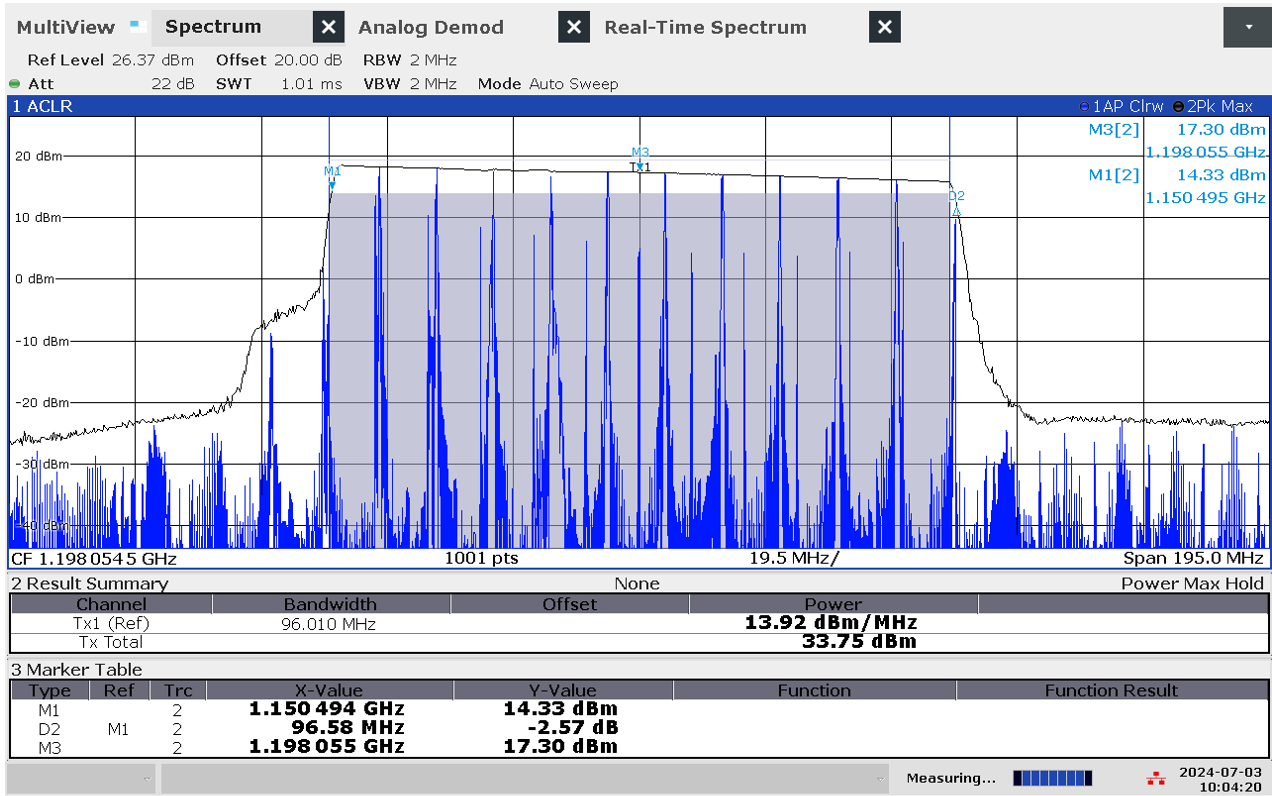
\includegraphics[width=\textwidth]{../graphics/appendixG/s2.1-2.png} 
\caption{Frequency and power measurement of jammer S2.1 on antenna 'L2'}\end{figure}\begin{figure}[H]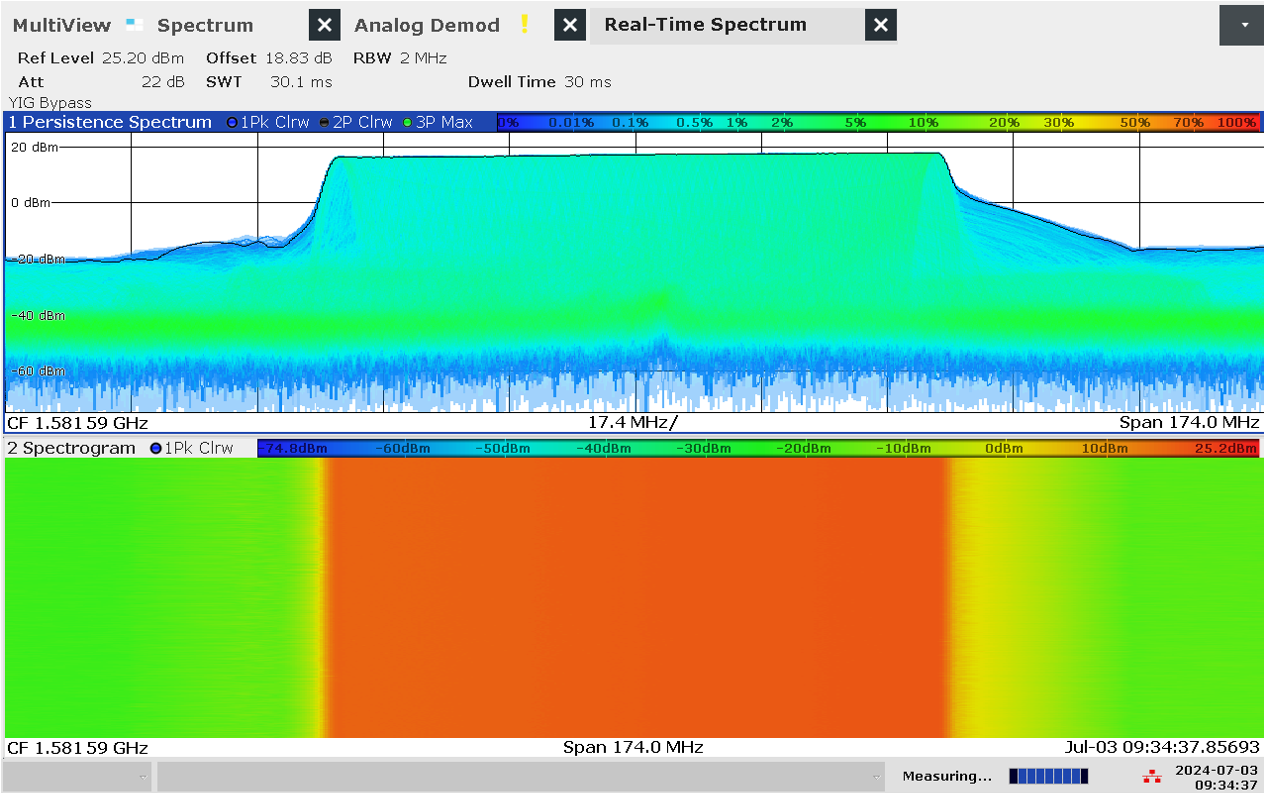
\includegraphics[width=\textwidth]{../graphics/appendixG/s2.1-3.png} 
\caption{Real-time persistence and spectrogram measurement of jammer S2.1 on antenna 'L1'}\end{figure}\begin{figure}[H]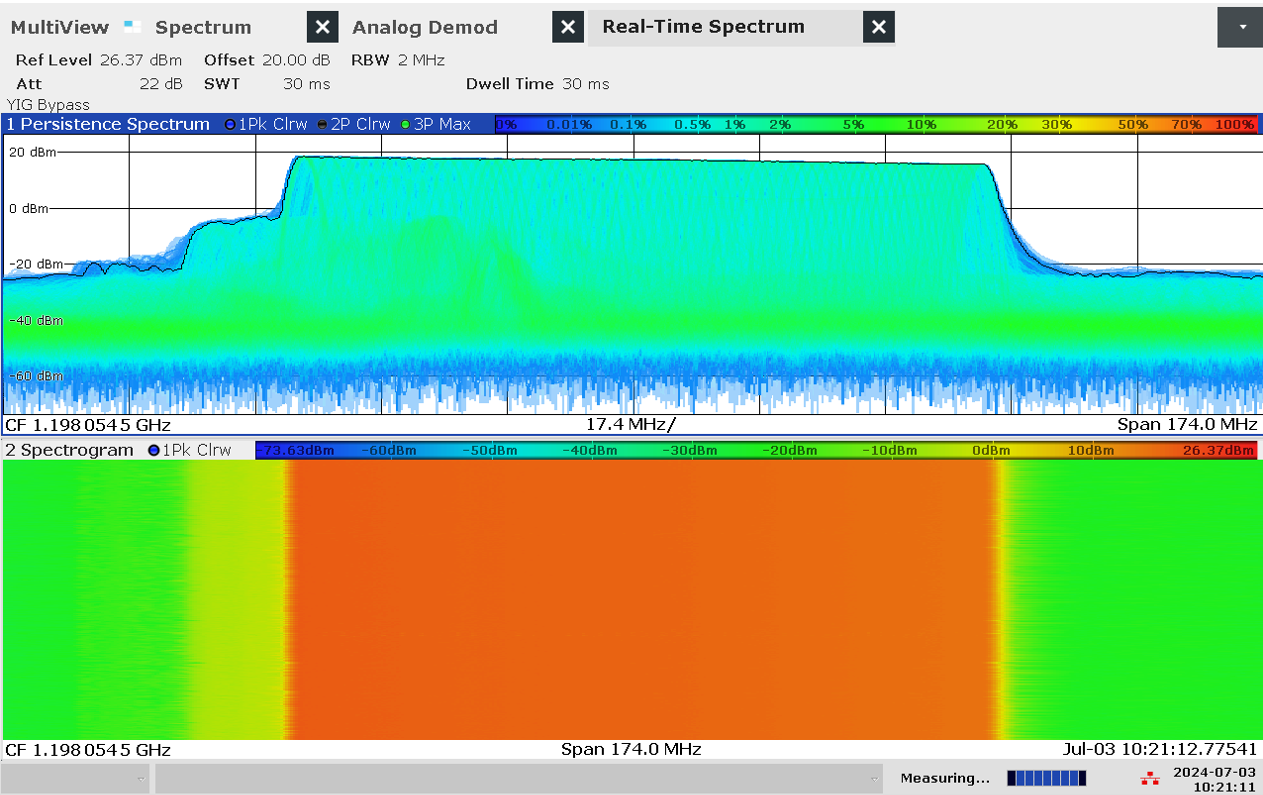
\includegraphics[width=\textwidth]{../graphics/appendixG/s2.1-4.png} 
\caption{Real-time persistence and spectrogram measurement of jammer S2.1 on antenna 'L2'}\end{figure}\begin{figure}[H]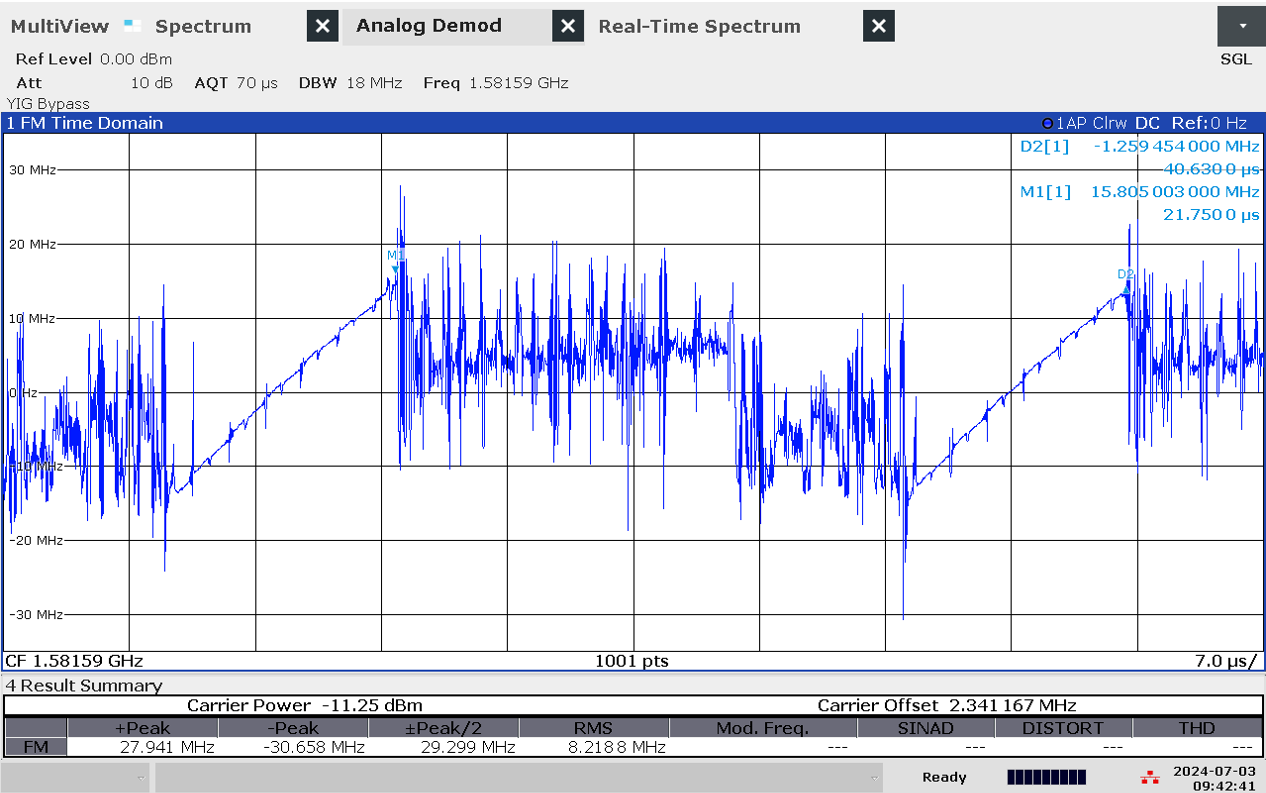
\includegraphics[width=\textwidth]{../graphics/appendixG/s2.1-5.png} 
\caption{Time domain (analog demod) measurement of jammer S2.1 on antenna 'L1'}\end{figure}\begin{figure}[H]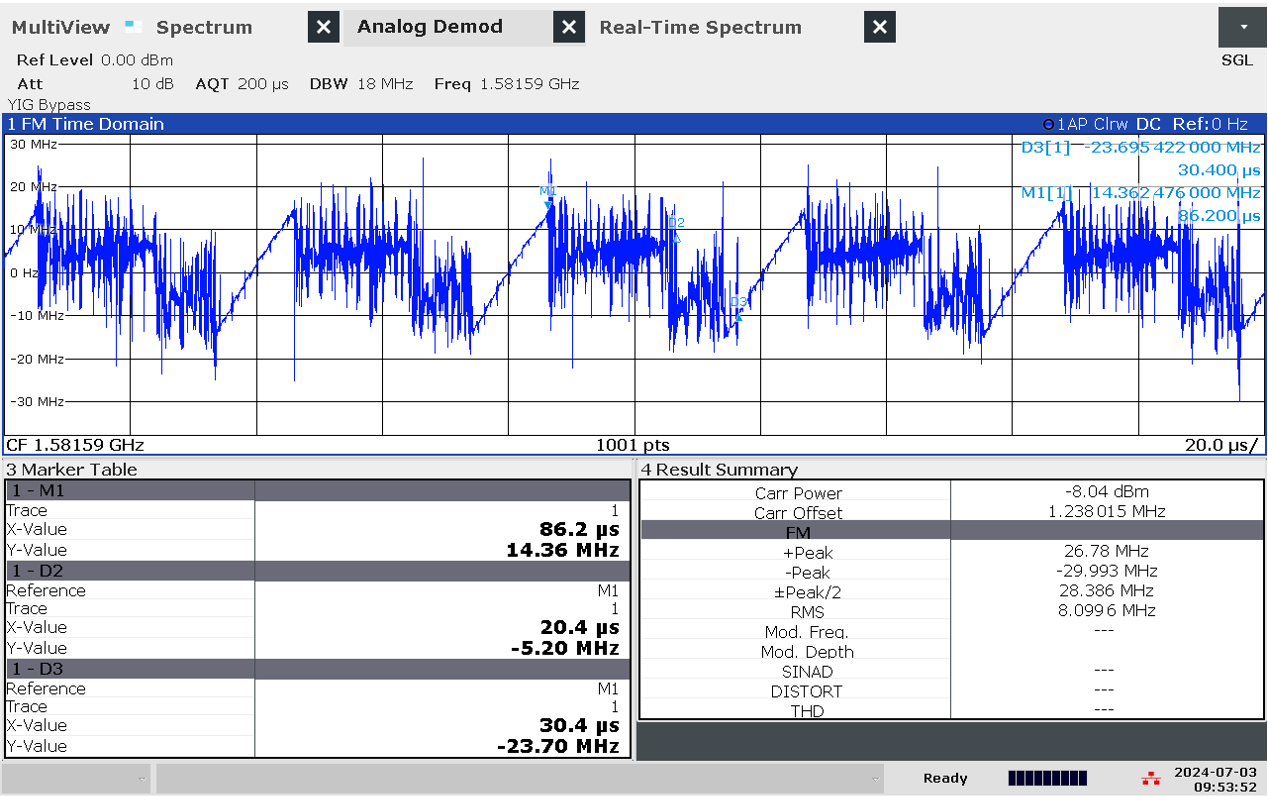
\includegraphics[width=\textwidth]{../graphics/appendixG/s2.1-6.png} 
\caption{Time domain (analog demod) measurement with wider span of jammer S2.1 on antenna 'L1'}\end{figure}\begin{figure}[H]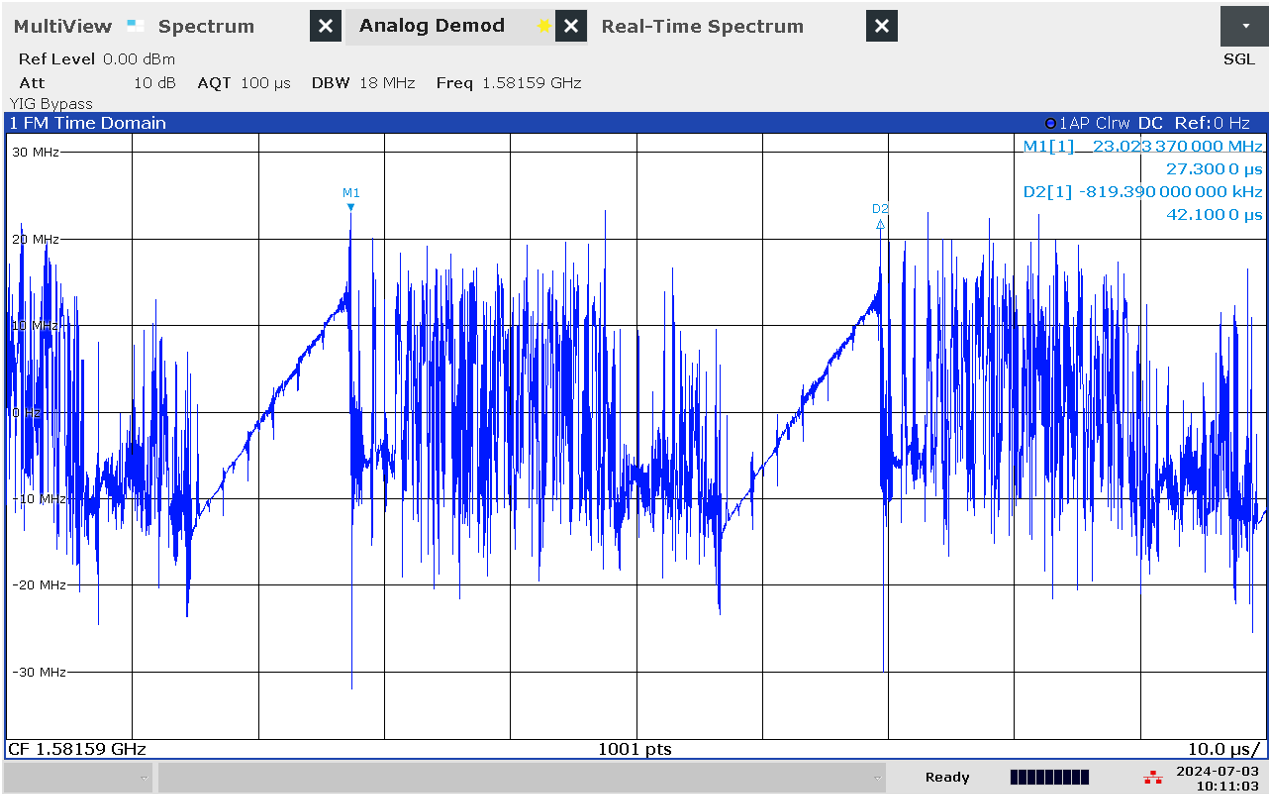
\includegraphics[width=\textwidth]{../graphics/appendixG/s2.1-7.png} 
\caption{Time domain (analog demod) measurement of jammer S2.1 on antenna 'L2'}\end{figure}\subsection{Technical details on low-power jammer 'S2.2'}
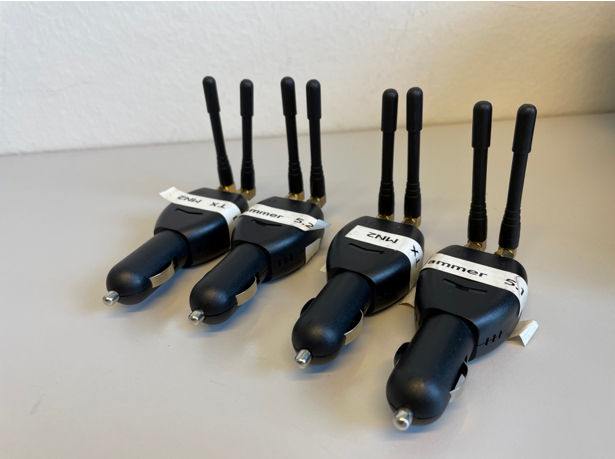
\includegraphics[scale=0.4]{../graphics/appendixG/s2.1-photo.png}\\ \\ 
The jammer S2.2 belongs to the 'Cigarette jammer' category of jammers. Such jammers are often installed in the cigarette lighter outlet in cars. They are intended to cover the car, and a given radius around the car. \\S2.2 is a two-antenna, so-called 'L1+L2', jammer, disrupting both the upper and lower L-band.\\
\begin{table}[H]\centering
\begin{tabular}{|c|c|c|c|c|c|c|c|}\rowcolor[HTML]{C0C0C0} 
\hline
\makecell{Antenna} & \makecell{Centre frequency\\{[MHz]}} & \makecell{Bandwidth\\{[MHz]}} & \makecell{PSD\\{[dBm/MHz]}} & \makecell{TX total\\{[dBm]}} & \makecell{CF max\\{[dBm]}} & \makecell{Sweep rate\\{[µs]}} & \makecell{Modulation}\\ 
\hline
\makecell{L1} & \makecell{1580.86} & \makecell{87.69} & \makecell{12.82} & \makecell{32.25} & \makecell{16.17} & \makecell{40.7} & \makecell{Sawtooth+burst}\\ 
\hline
\makecell{L2} & \makecell{1207.55} & \makecell{102.04} & \makecell{11.95} & \makecell{32.04} & \makecell{17.02} & \makecell{41.0} & \makecell{Sawtooth+burst}\\ 
\hline\end{tabular}\caption{Technical characteristics of S2.2 jammer}\label{table:tech_char_S2.2}\end{table}
\begin{figure}[H]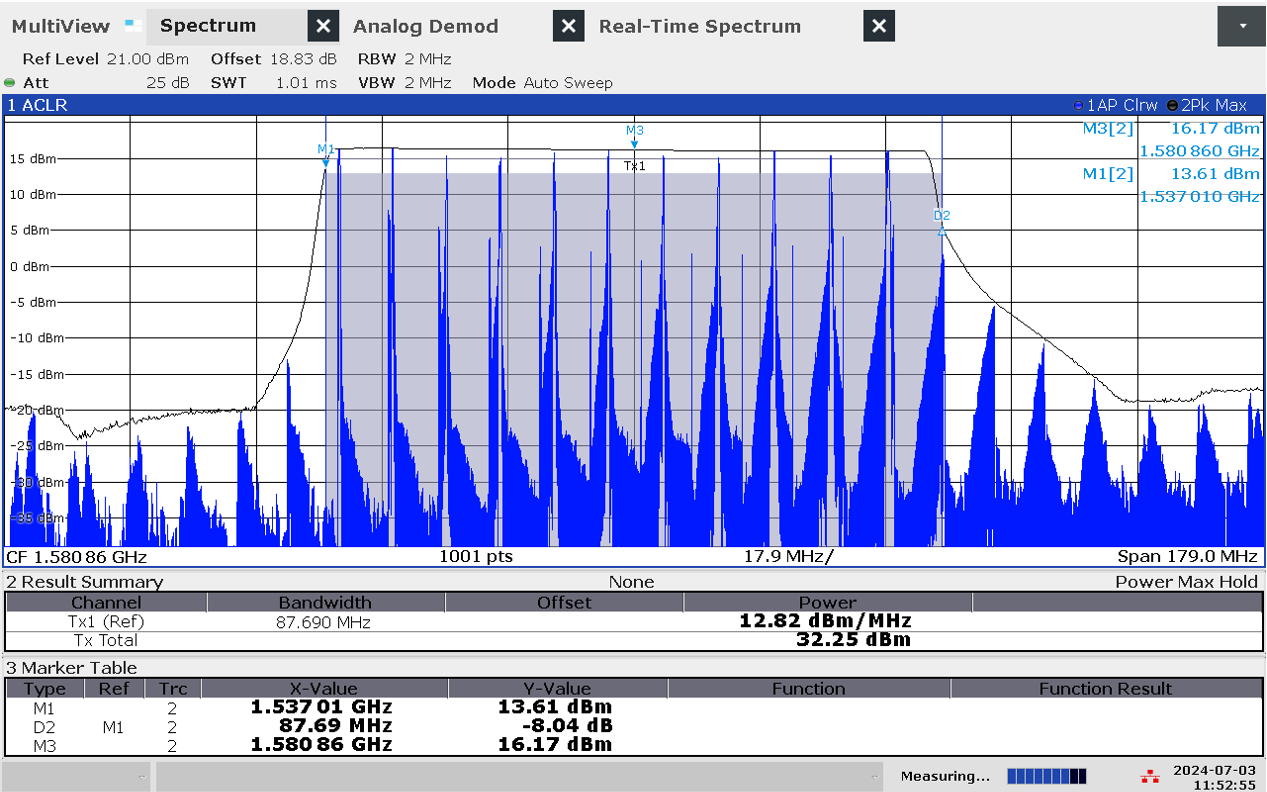
\includegraphics[width=\textwidth]{../graphics/appendixG/s2.2-1.png} 
\caption{Frequency and power measurement of jammer S2.2 on antenna 'L1'}\end{figure}\begin{figure}[H]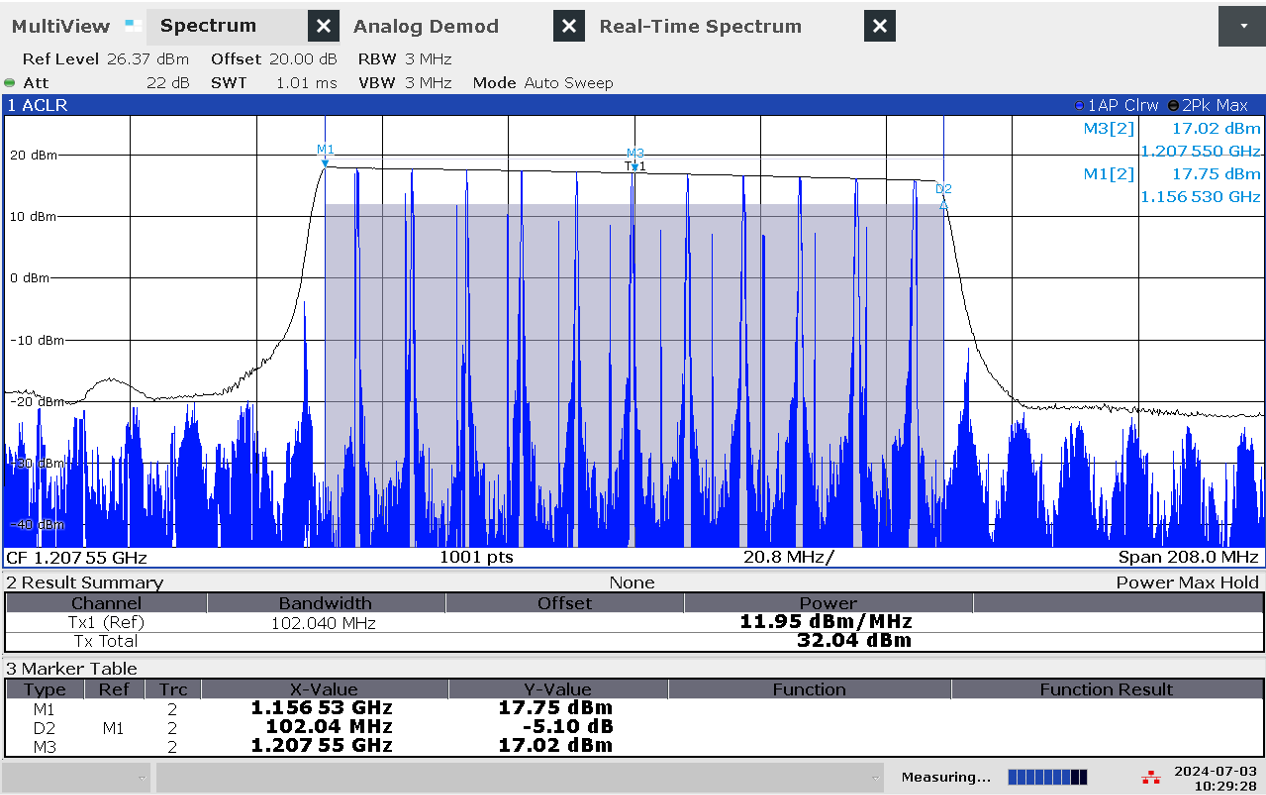
\includegraphics[width=\textwidth]{../graphics/appendixG/s2.2-2.png} 
\caption{Frequency and power measurement of jammer S2.2 on antenna 'L2'}\end{figure}\begin{figure}[H]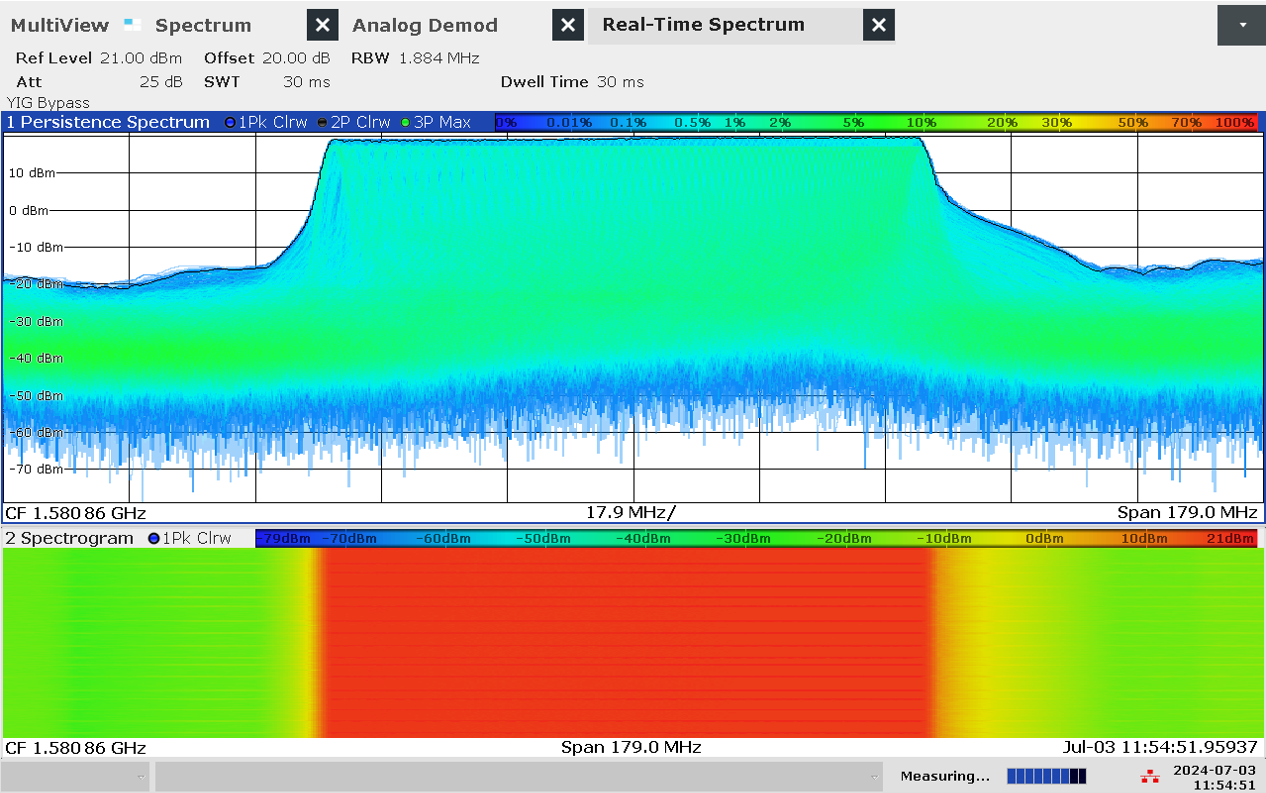
\includegraphics[width=\textwidth]{../graphics/appendixG/s2.2-3.png} 
\caption{Real-time persistence and spectrogram measurement of jammer S2.2 on antenna 'L1'}\end{figure}\begin{figure}[H]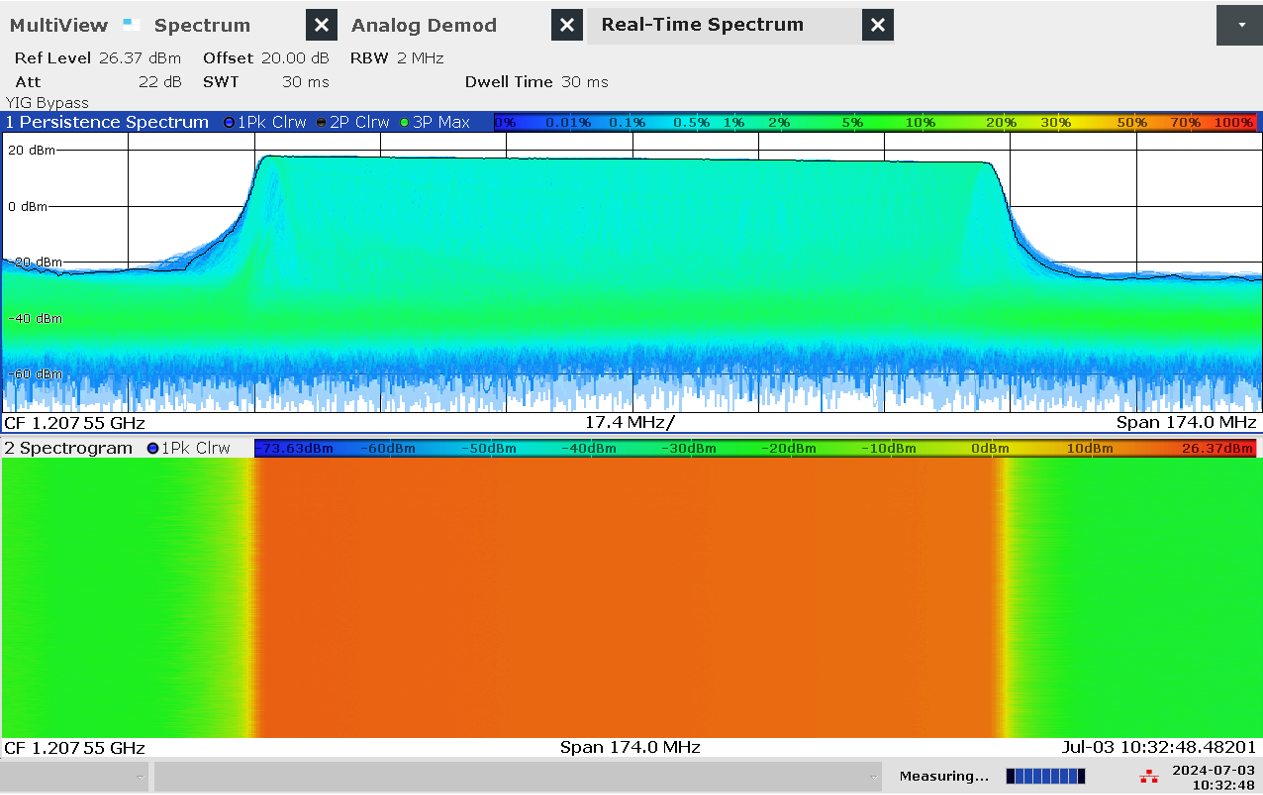
\includegraphics[width=\textwidth]{../graphics/appendixG/s2.2-4.png} 
\caption{Real-time persistence and spectrogram measurement of jammer S2.2 on antenna 'L2'}\end{figure}\begin{figure}[H]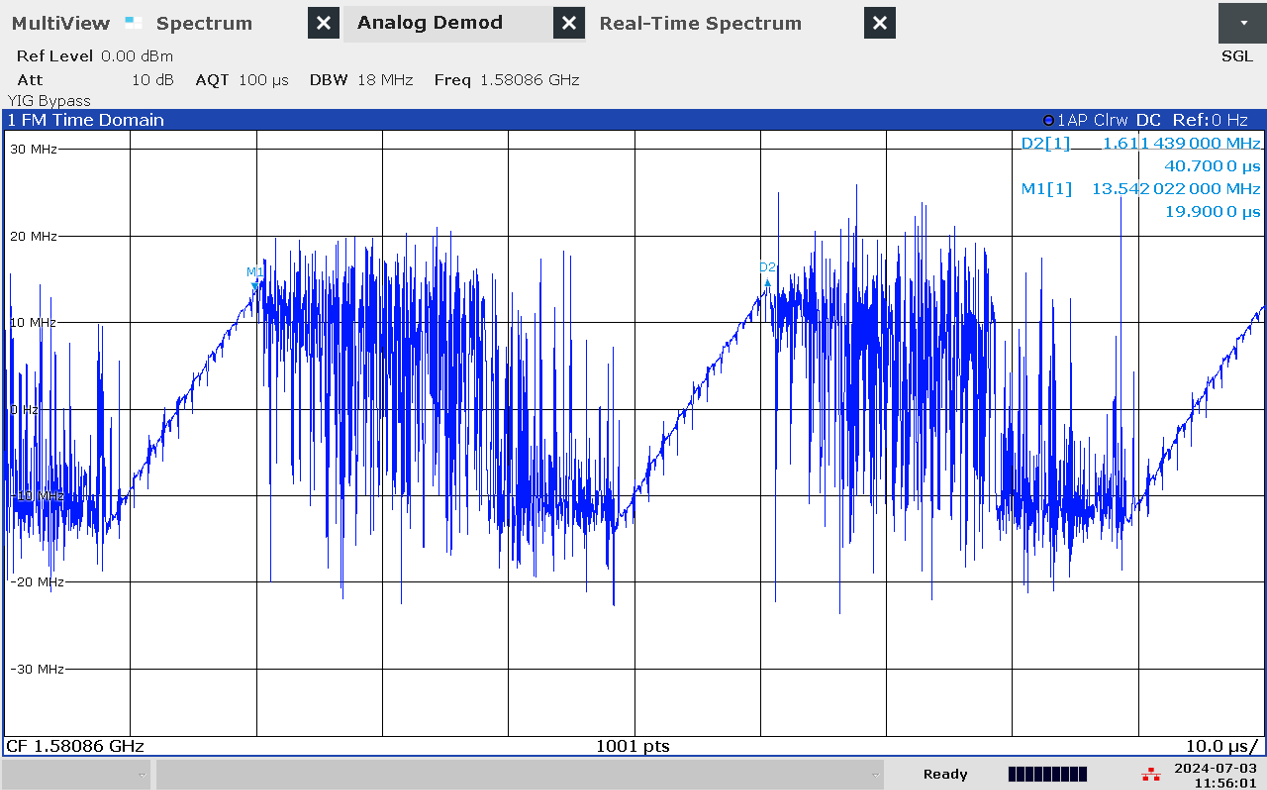
\includegraphics[width=\textwidth]{../graphics/appendixG/s2.2-5.png} 
\caption{Time domain (analog demod) measurement of jammer S2.2 on antenna 'L1'}\end{figure}\begin{figure}[H]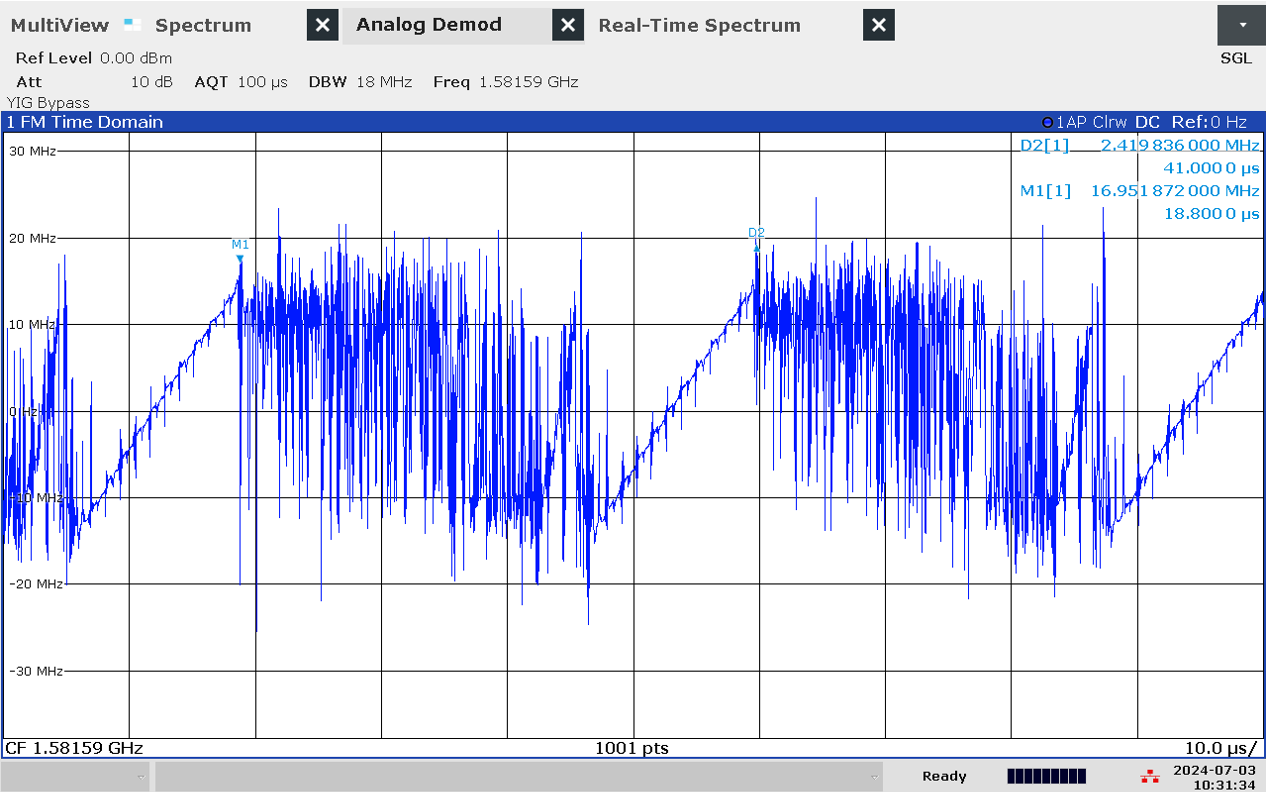
\includegraphics[width=\textwidth]{../graphics/appendixG/s2.2-6.png} 
\caption{Time domain (analog demod) measurement of jammer S2.2 on antenna 'L2'}\end{figure}\subsection{Technical details on low-power jammer 'S2.3'}
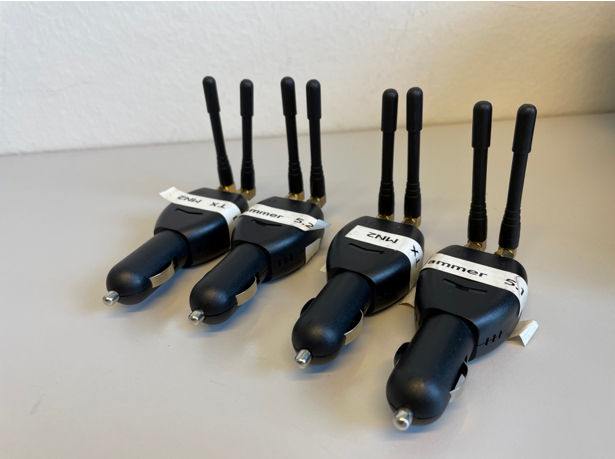
\includegraphics[scale=0.4]{../graphics/appendixG/s2.1-photo.png}\\ \\ 
The jammer S2.3 belongs to the 'Cigarette jammer' category of jammers. Such jammers are often installed in the cigarette lighter outlet in cars. They are intended to cover the car, and a given radius around the car. \\S2.3 is a two-antenna, so-called 'L1+L2', jammer, disrupting both the upper and lower L-band.\\
\begin{table}[H]\centering
\begin{tabular}{|c|c|c|c|c|c|c|c|}\rowcolor[HTML]{C0C0C0} 
\hline
\makecell{Antenna} & \makecell{Centre frequency\\{[MHz]}} & \makecell{Bandwidth\\{[MHz]}} & \makecell{PSD\\{[dBm/MHz]}} & \makecell{TX total\\{[dBm]}} & \makecell{CF max\\{[dBm]}} & \makecell{Sweep rate\\{[µs]}} & \makecell{Modulation}\\ 
\hline
\makecell{L1} & \makecell{1586.65} & \makecell{93.19} & \makecell{14.30} & \makecell{34.0} & \makecell{17.40} & \makecell{46.7} & \makecell{Sawtooth+burst}\\ 
\hline
\makecell{L2} & \makecell{1204.33} & \makecell{102.05} & \makecell{12.01} & \makecell{32.1} & \makecell{17.06} & \makecell{50.5} & \makecell{Sawtooth+burst}\\ 
\hline\end{tabular}\caption{Technical characteristics of S2.3 jammer}\label{table:tech_char_S2.3}\end{table}
\begin{figure}[H]\includegraphics[width=\textwidth]{../graphics/appendixG/S2.3-1.png} 
\caption{Frequency and power measurement of jammer S2.3 on antenna 'L1'}\end{figure}\begin{figure}[H]\includegraphics[width=\textwidth]{../graphics/appendixG/S2.3-2.png} 
\caption{Frequency and power measurement of jammer S2.3 on antenna 'L2'}\end{figure}\begin{figure}[H]\includegraphics[width=\textwidth]{../graphics/appendixG/S2.3-3.png} 
\caption{Real-time persistence and spectrogram measurement of jammer S2.3 on antenna 'L1'}\end{figure}\begin{figure}[H]\includegraphics[width=\textwidth]{../graphics/appendixG/S2.3-4.png} 
\caption{Real-time persistence and spectrogram measurement of jammer S2.3 on antenna 'L2'}\end{figure}\begin{figure}[H]\includegraphics[width=\textwidth]{../graphics/appendixG/S2.3-5.png} 
\caption{Time domain (analog demod) measurement of jammer S2.3 on antenna 'L1'}\end{figure}\begin{figure}[H]\includegraphics[width=\textwidth]{../graphics/appendixG/S2.3-6.png} 
\caption{Time domain (analog demod) measurement of jammer S2.3 on antenna 'L2'}\end{figure}\subsection{Technical details on low-power jammer 'S2.4'}
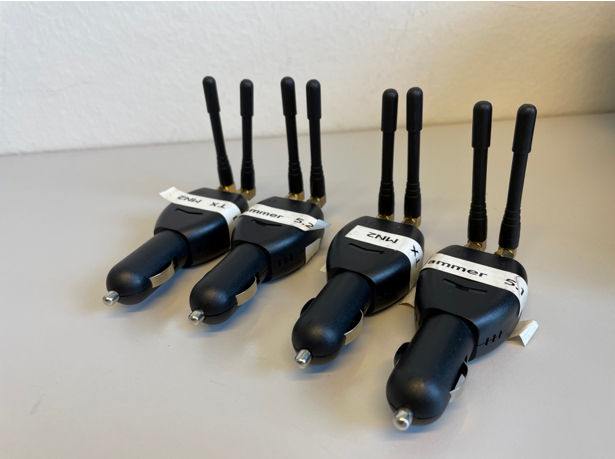
\includegraphics[scale=0.4]{../graphics/appendixG/s2.1-photo.png}\\ \\ 
The jammer S2.4 belongs to the 'Cigarette jammer' category of jammers. Such jammers are often installed in the cigarette lighter outlet in cars. They are intended to cover the car, and a given radius around the car. \\S2.4 is a two-antenna, so-called 'L1+L2', jammer, disrupting both the upper and lower L-band.\\
\begin{table}[H]\centering
\begin{tabular}{|c|c|c|c|c|c|c|c|}\rowcolor[HTML]{C0C0C0} 
\hline
\makecell{Antenna} & \makecell{Centre frequency\\{[MHz]}} & \makecell{Bandwidth\\{[MHz]}} & \makecell{PSD\\{[dBm/MHz]}} & \makecell{TX total\\{[dBm]}} & \makecell{CF max\\{[dBm]}} & \makecell{Sweep rate\\{[µs]}} & \makecell{Modulation}\\ 
\hline
\makecell{L1} & \makecell{1582.09} & \makecell{86.35} & \makecell{12.42} & \makecell{31.78} & \makecell{15.91} & \makecell{43.5} & \makecell{Sawtooth+burst}\\ 
\hline
\makecell{L2} & \makecell{1202.90} & \makecell{96.56} & \makecell{13.63} & \makecell{33.48} & \makecell{17.03} & \makecell{47.3} & \makecell{Sawtooth+burst}\\ 
\hline\end{tabular}\caption{Technical characteristics of S2.4 jammer}\label{table:tech_char_S2.4}\end{table}
\begin{figure}[H]\includegraphics[width=\textwidth]{../graphics/appendixG/S2.4-1.png} 
\caption{Frequency and power measurement of jammer S2.4 on antenna 'L1'}\end{figure}\begin{figure}[H]\includegraphics[width=\textwidth]{../graphics/appendixG/S2.4-2.png} 
\caption{Frequency and power measurement of jammer S2.4 on antenna 'L2'}\end{figure}\begin{figure}[H]\includegraphics[width=\textwidth]{../graphics/appendixG/S2.4-3.png} 
\caption{Real-time persistence and spectrogram measurement of jammer S2.4 on antenna 'L1'}\end{figure}\begin{figure}[H]\includegraphics[width=\textwidth]{../graphics/appendixG/S2.4-4.png} 
\caption{Real-time persistence and spectrogram measurement of jammer S2.4 on antenna 'L2'}\end{figure}\begin{figure}[H]\includegraphics[width=\textwidth]{../graphics/appendixG/S2.4-5.png} 
\caption{Time domain (analog demod) measurement of jammer S2.4 on antenna 'L1'}\end{figure}\begin{figure}[H]\includegraphics[width=\textwidth]{../graphics/appendixG/S2.4-6.png} 
\caption{Time domain (analog demod) measurement of jammer S2.4 on antenna 'L2'}\end{figure}\subsection{Technical details on low-power jammer 'U1.1 to U1.4'}
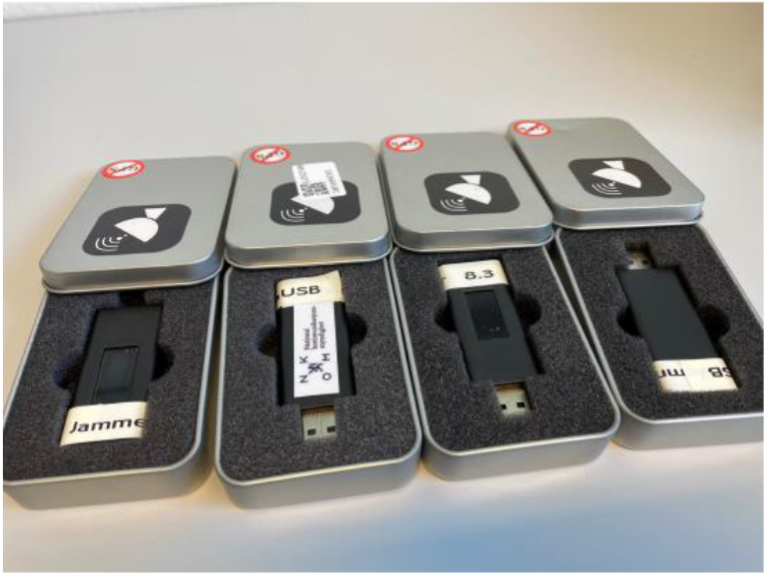
\includegraphics[scale=0.4]{../graphics/appendixG/u1.1-photo.png}\\ \\ 
USB jammers is category of jammers that is often installed in the USB outlet. The are intended to cover a small radius. These particular jammers suggest in the LED screen that they jam two bands, although this is not the case\\
\begin{table}[H]\centering
\begin{tabular}{|c|c|c|c|c|c|c|}\rowcolor[HTML]{C0C0C0} 
\hline
\makecell{Centre frequency\\{[MHz]}} & \makecell{Bandwidth\\{[MHz]}} & \makecell{PSD\\{[dBm/MHz]}} & \makecell{TX total\\{[dBm]}} & \makecell{CF max\\{[dBm]}} & \makecell{Sweep rate\\{[µs]}} & \makecell{Modulation}\\ 
\hline
\makecell{1590-1600} & \makecell{70-80} & \makecell{N/A} & \makecell{N/A} & \makecell{N/A} & \makecell{5-8} & \makecell{Sawtooth}\\ 
\hline\end{tabular}\caption{Technical characteristics of U1.1-U1.4 jammer}\label{table:tech_char_U1.1-U1.4}\end{table}
\begin{figure}[H]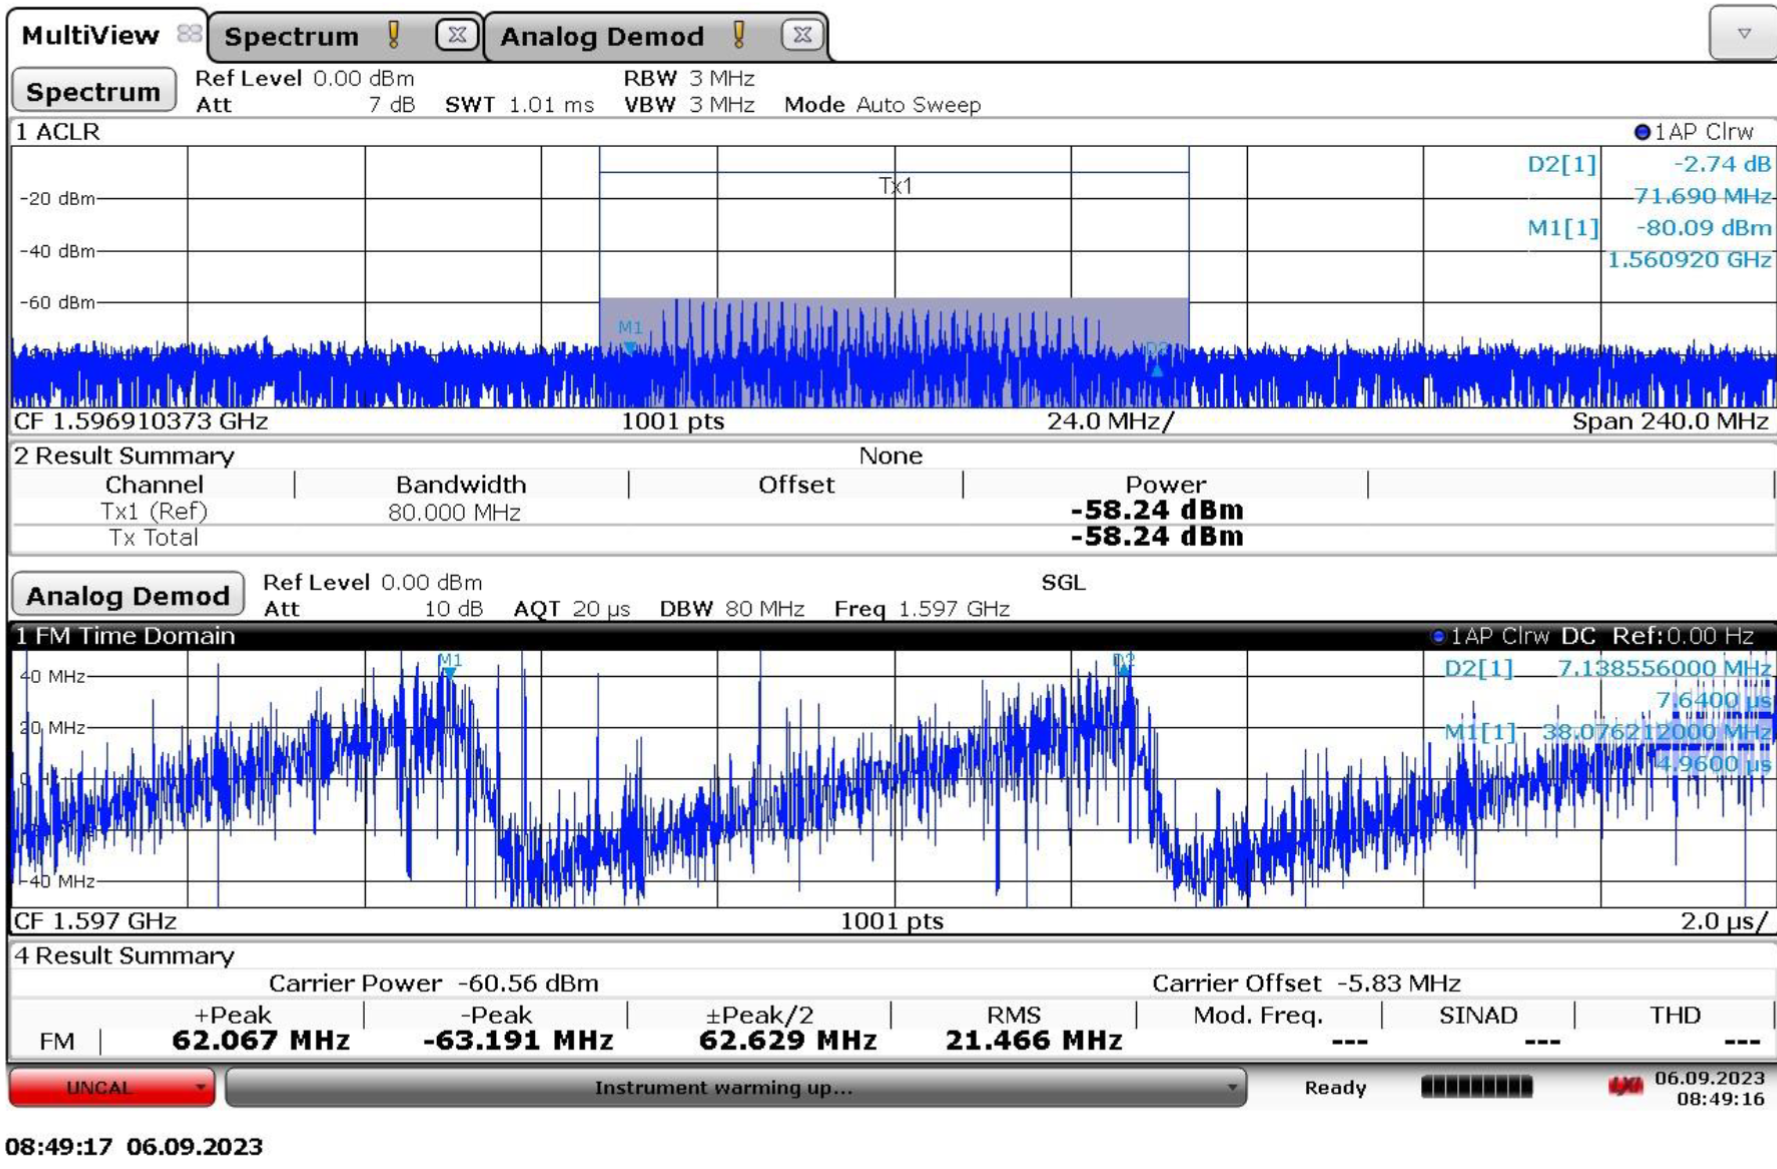
\includegraphics[width=\textwidth]{../graphics/appendixG/u1.1-1.png} 
\caption{Example measurement of a U1.1 - U1.4 jammer}\end{figure}\subsection{Technical details on low-power jammer 'H1.1'}
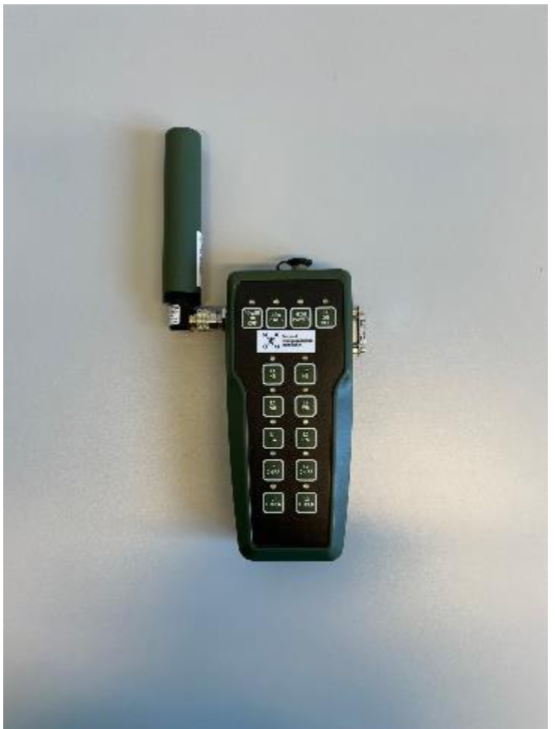
\includegraphics[scale=0.4]{../graphics/appendixG/h1.1-photo.png}\\ \\ 
The jammer H1.1 belongs to the 'Handheld category' of jammers. It is a medium weight battery driven jammer with a configuration panel for operation: multi-frequency and multi-modulation for both low and high output power. Its commercially available for military training purposes as Novatel's NEAT-jammer. Antenna has TNC-connector.\\H1.1 is a one-antenna, yet multi-frequency, jammer, therefore a so-called 'L1+L2', disrupting parts of both the upper and lower L-band. Jammer (H1.4, H1.5, H1.6 and H1.7) are the same type as H1.1, but the measuremensts are all done on H1.1. \\\\ Configuration choices are (as provided by the producer):\\ - Centre frequency: 1575.42 MHz and 1227.6 MHz\\ - Estimated output power: low power -5 dBm, high power 20 dBm\\ - Type of modulation: narrow band (NB), wide band (WB), continuous wave (CW), chirp/sweep and other (optional to program)\\\\ In the 2024 measurements below, bandwidth is defined as\\ - main lobe in PRN signal\\ - 3 dB from local (identifiable) maxima\\
\begin{table}[H]\centering
\begin{tabular}{|c|c|c|c|c|c|c|c|}\rowcolor[HTML]{C0C0C0} 
\hline
\makecell{Antenna\\configuration} & \makecell{Centre frequency\\{[MHz]}} & \makecell{Bandwidth\\{[MHz]}} & \makecell{PSD\\{[dBm/MHz]}} & \makecell{TX total\\{[dBm]}} & \makecell{CF max\\{[dBm]}} & \makecell{Sweep rate\\{[µs]}} & \makecell{Modulation}\\ 
\hline
\makecell{L1. NB. HIGH PWR} & \makecell{1575.42} & \makecell{2.05} & \makecell{17.52} & \makecell{20.63} & \makecell{11.07} & \makecell{N/A} & \makecell{PRN\\(spreading code of 1 MHz)}\\ 
\hline
\makecell{L1. WB. HIGH PWR} & \makecell{1575.40} & \makecell{20.03} & \makecell{8.20} & \makecell{21.25} & \makecell{11.43} & \makecell{N/A} & \makecell{PRN\\(spreading code of 10 MHz)}\\ 
\hline
\makecell{L1. CW. HIGH PWR} & \makecell{1575.42} & \makecell{0.103} & \makecell{22.50} & \makecell{12.62} & \makecell{13.67} & \makecell{N/A} & \makecell{CW}\\ 
\hline
\makecell{L1. CHIRP. HIGH PWR} & \makecell{1575.60} & \makecell{18.75} & \makecell{3.10} & \makecell{15.83} & \makecell{-5.73} & \makecell{10.42} & \makecell{Sawtooth}\\ 
\hline
\makecell{L1. NB. LOW PWR} & \makecell{1575.42} & \makecell{2.05} & \makecell{-12.84} & \makecell{-9.73} & \makecell{-19.35} & \makecell{N/A} & \makecell{PRN\\(spreading code of 1 MHz)}\\ 
\hline
\makecell{L1. WB. LOW PWR} & \makecell{1575.40} & \makecell{19.93} & \makecell{-21.66} & \makecell{-8.66} & \makecell{-17.91} & \makecell{N/A} & \makecell{PRN\\(spreading code of 10 MHz)}\\ 
\hline
\makecell{L1. CW. LOW PWR} & \makecell{1575.42} & \makecell{0.10} & \makecell{-7.55} & \makecell{-17.46} & \makecell{-16.37} & \makecell{N/A} & \makecell{CW}\\ 
\hline
\makecell{L1. CHIRP. LOW PWR} & \makecell{1575.60} & \makecell{18.75} & \makecell{-27.03} & \makecell{-14.31} & \makecell{-35.65} & \makecell{10.46} & \makecell{Sawtooth}\\ 
\hline
\makecell{L2. NB. HIGH PWR} & \makecell{1227.42} & \makecell{2.049} & \makecell{18.73} & \makecell{21.84} & \makecell{12.17} & \makecell{N/A} & \makecell{PRN\\(spreading code of 1 MHz)}\\ 
\hline
\makecell{L2. WB. HIGH PWR} & \makecell{1227.36} & \makecell{20.30} & \makecell{9.27} & \makecell{22.34} & \makecell{12.09} & \makecell{N/A} & \makecell{PRN\\(spreading code of 10 MHz)}\\ 
\hline
\makecell{L2. CW. HIGH PWR} & \makecell{1227.42} & \makecell{0.10} & \makecell{23.96} & \makecell{14.13} & \makecell{15.17} & \makecell{N/A} & \makecell{CW}\\ 
\hline
\makecell{L2. CHIRP. HIGH PWR} & \makecell{1227.22} & \makecell{18.79} & \makecell{4.98} & \makecell{17.72} & \makecell{-4.11} & \makecell{10.4} & \makecell{Sawtooth}\\ 
\hline
\makecell{L2. NB. LOW PWR} & \makecell{1227.42} & \makecell{2.05} & \makecell{-11.20} & \makecell{-8.09} & \makecell{-17.79} & \makecell{N/A} & \makecell{PRN\\(spreading code of 1 MHz)}\\ 
\hline
\makecell{L2. WB. LOW PWR} & \makecell{1227.36} & \makecell{20.30} & \makecell{-20.39} & \makecell{-7.32} & \makecell{-17.41} & \makecell{N/A} & \makecell{PRN\\(spreading code of 10 MHz)}\\ 
\hline
\makecell{L2. CW. LOW PWR} & \makecell{1227.42} & \makecell{0.10} & \makecell{-5.98} & \makecell{-15.81} & \makecell{-14.77} & \makecell{N/A} & \makecell{CW}\\ 
\hline
\makecell{L2. CHIRP. LOW PWR} & \makecell{1227.22} & \makecell{18.76} & \makecell{-24.97} & \makecell{-12.23} & \makecell{-33.98} & \makecell{10.4} & \makecell{Sawtooth}\\ 
\hline\end{tabular}\caption{Technical characteristics of H1.1 jammer}\label{table:tech_char_H1.1}\end{table}
\begin{figure}[H]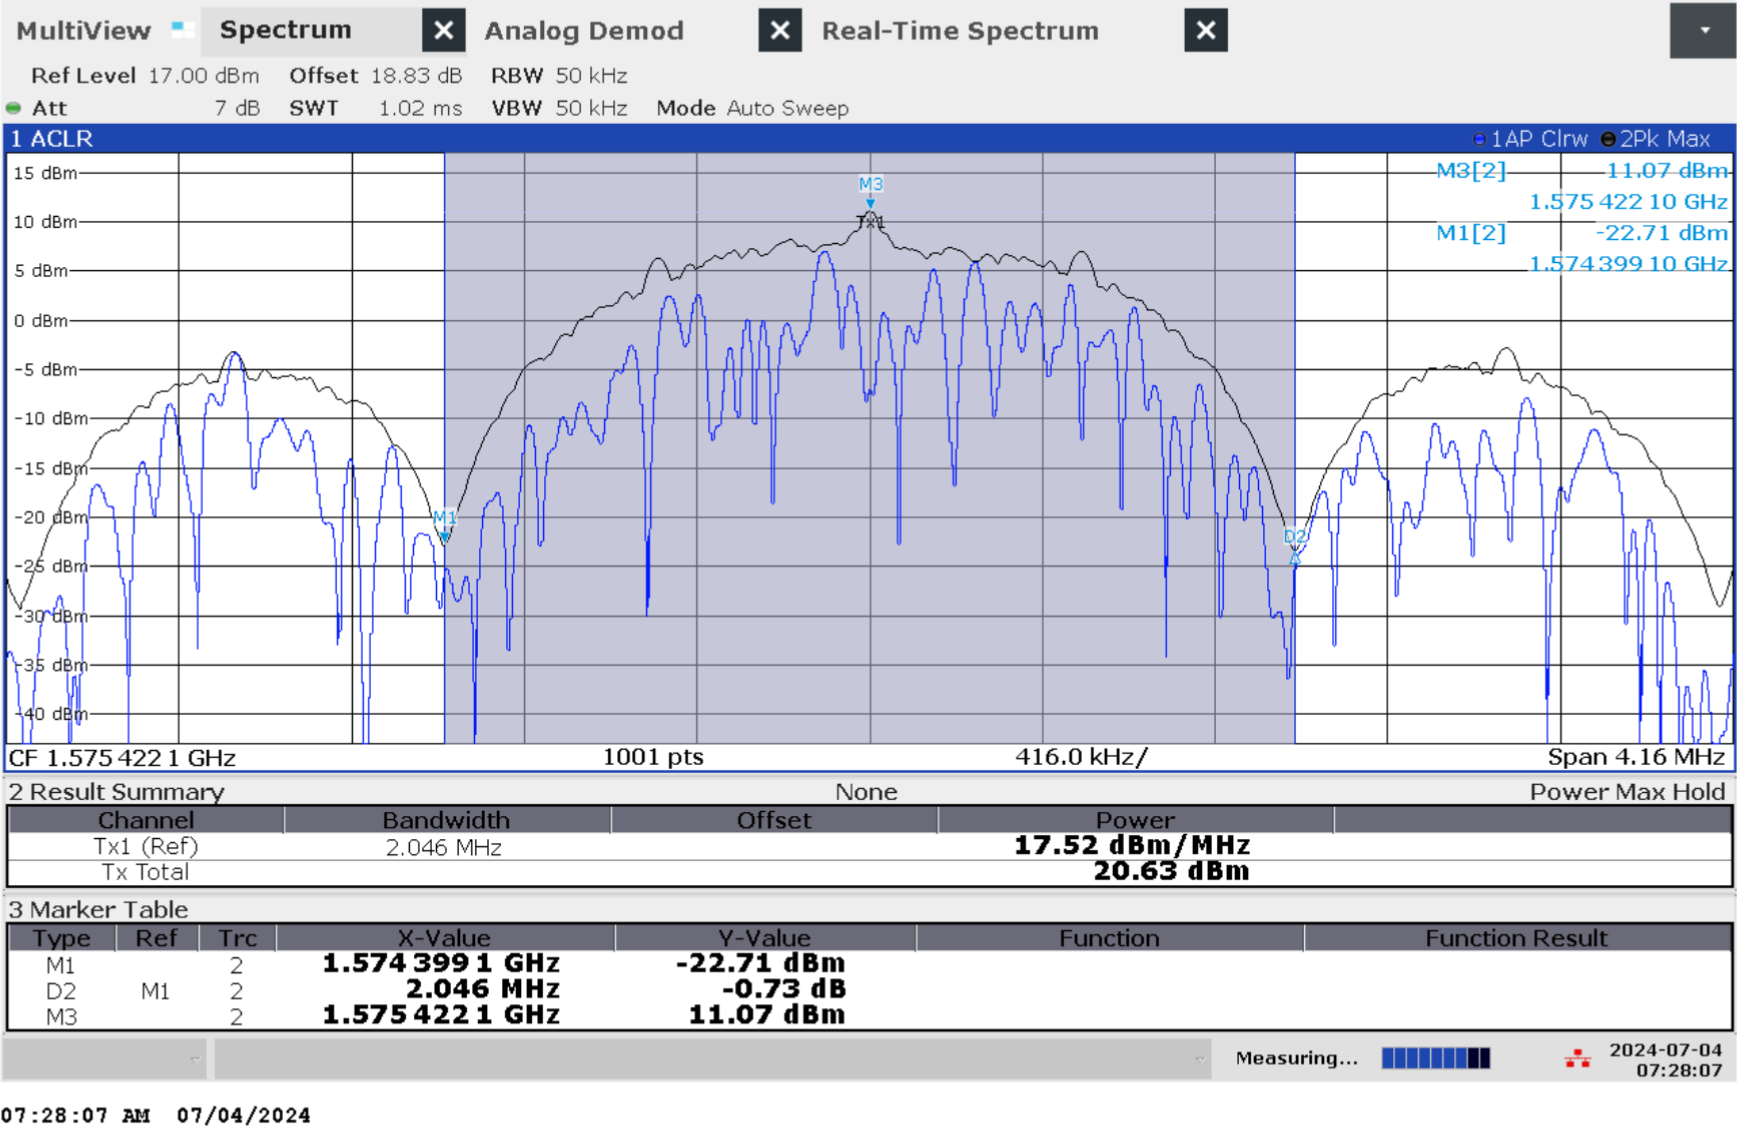
\includegraphics[width=\textwidth]{../graphics/appendixG/h1.1-1.png} 
\caption{Frequency and power measurement of jammer H1.1 with antenna configuration L1 Narrow band High Power (NB HIGH PWR)}\end{figure}\begin{figure}[H]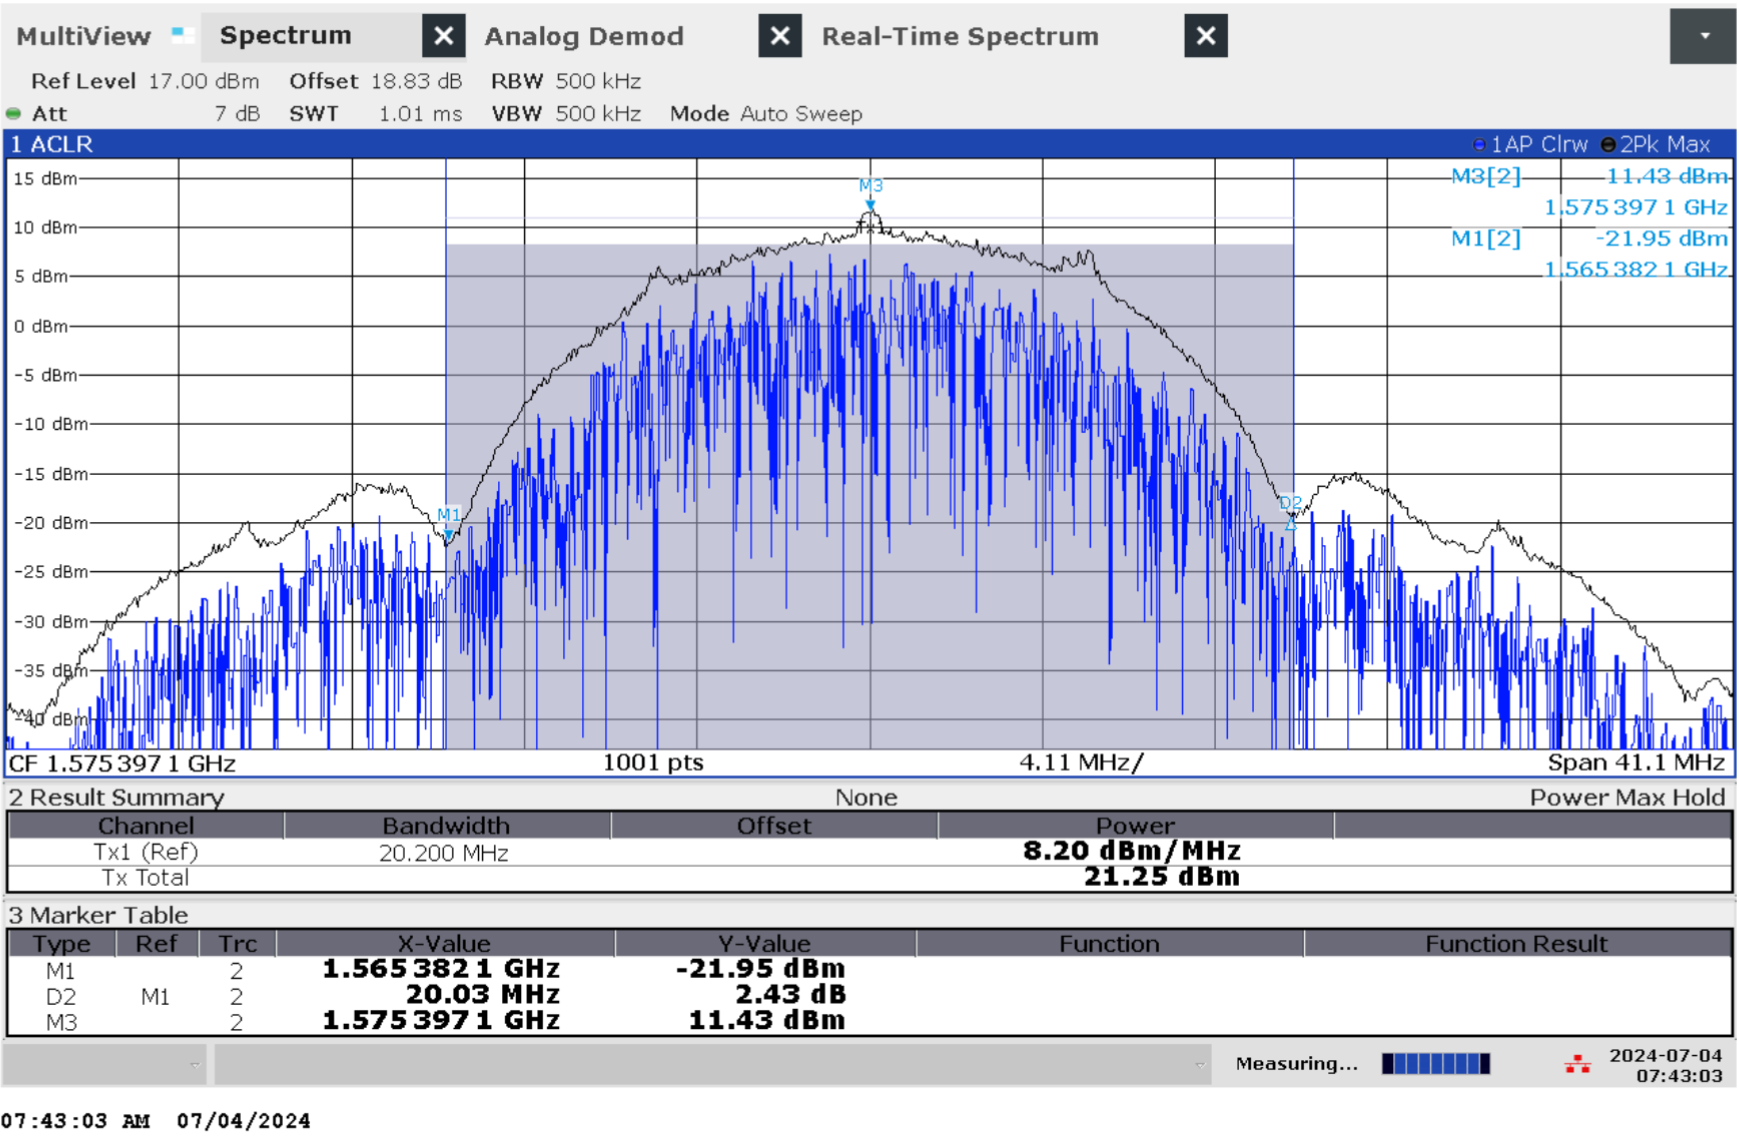
\includegraphics[width=\textwidth]{../graphics/appendixG/h1.1-2.png} 
\caption{Frequency and power measurement of jammer H1.1 with antenna configuration L1 Wide band High Power (WB HIGH PWR)}\end{figure}\begin{figure}[H]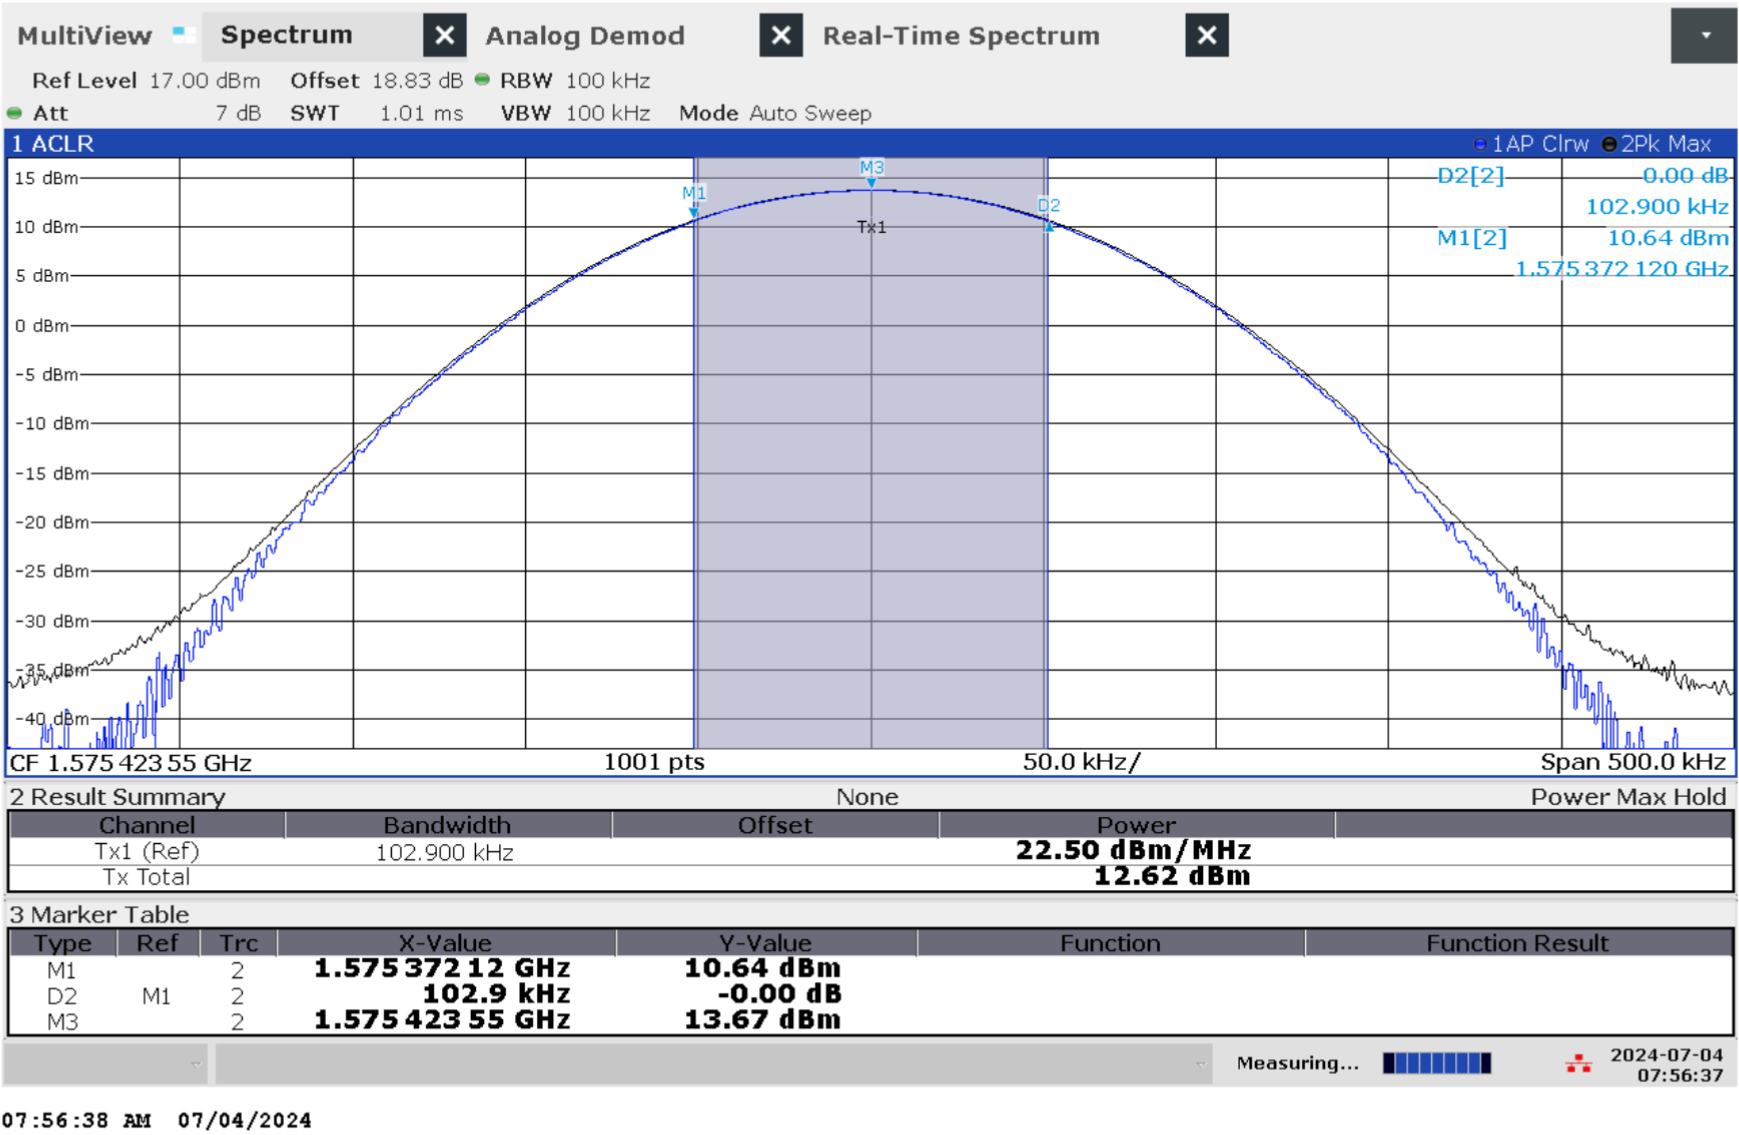
\includegraphics[width=\textwidth]{../graphics/appendixG/h1.1-3.png} 
\caption{Frequency and power measurement of jammer H1.1 with antenna configuration L1 Continuous Wave band High Power (CW HIGH PWR)}\end{figure}\begin{figure}[H]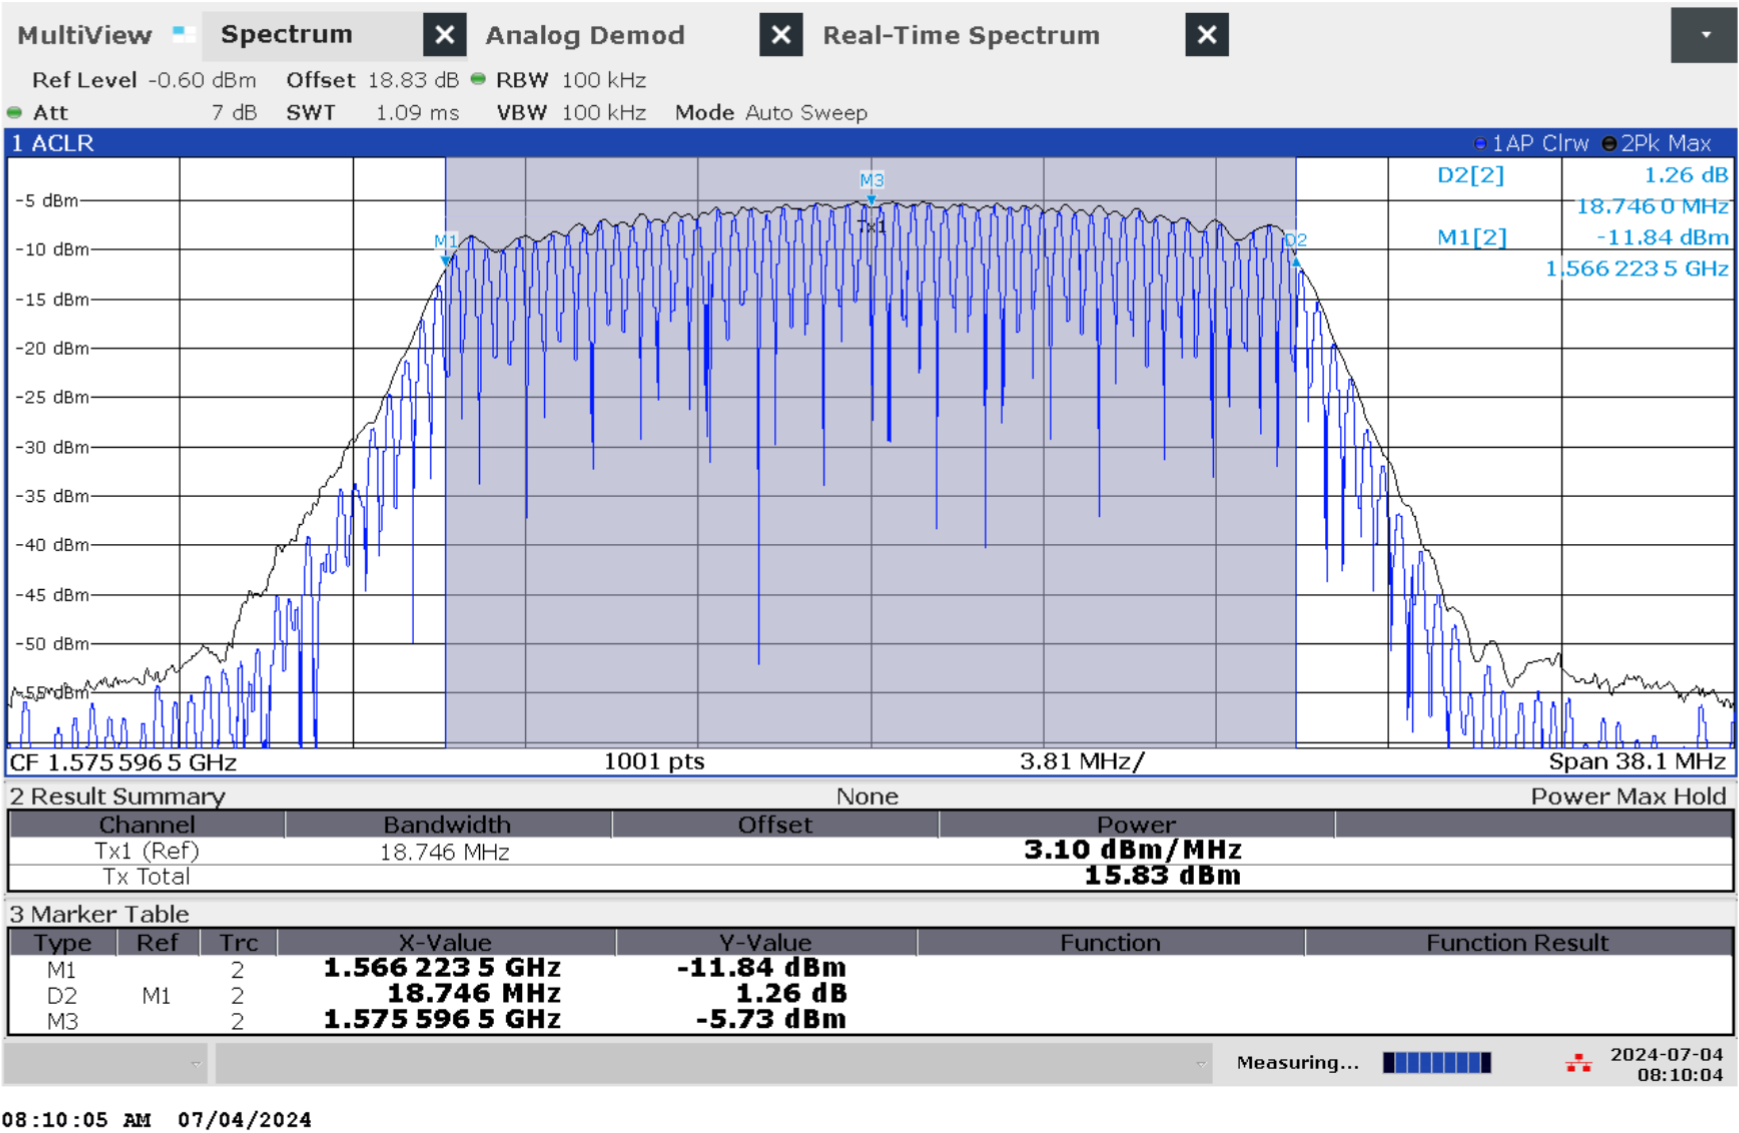
\includegraphics[width=\textwidth]{../graphics/appendixG/h1.1-4.png} 
\caption{Frequency and power measurement of jammer H1.1 with antenna configuration L1 Chirp High Power (CHIRP HIGH PWR)}\end{figure}\begin{figure}[H]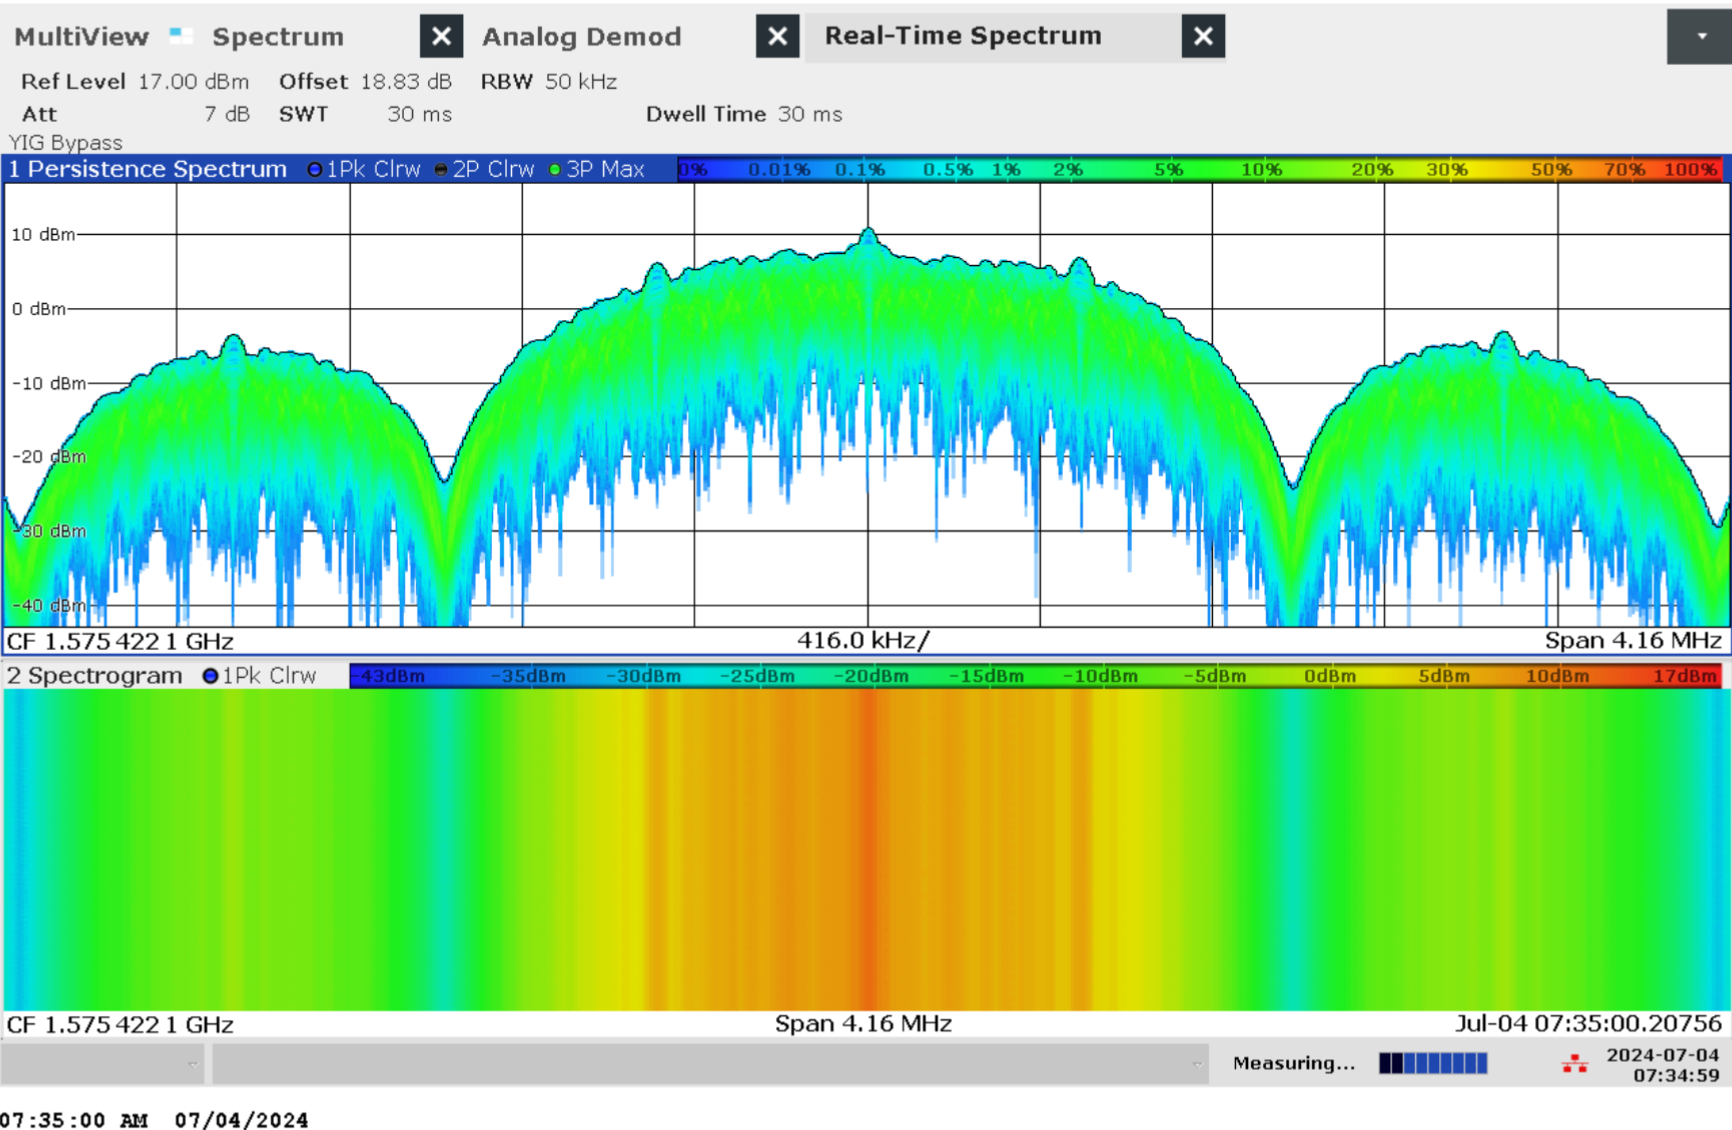
\includegraphics[width=\textwidth]{../graphics/appendixG/h1.1-5.png} 
\caption{Real-time persistence and spectrogram measurement of jammer H1.1 with antenna configuration L1 Narrow band High Power (NB HIGH PWR)}\end{figure}\begin{figure}[H]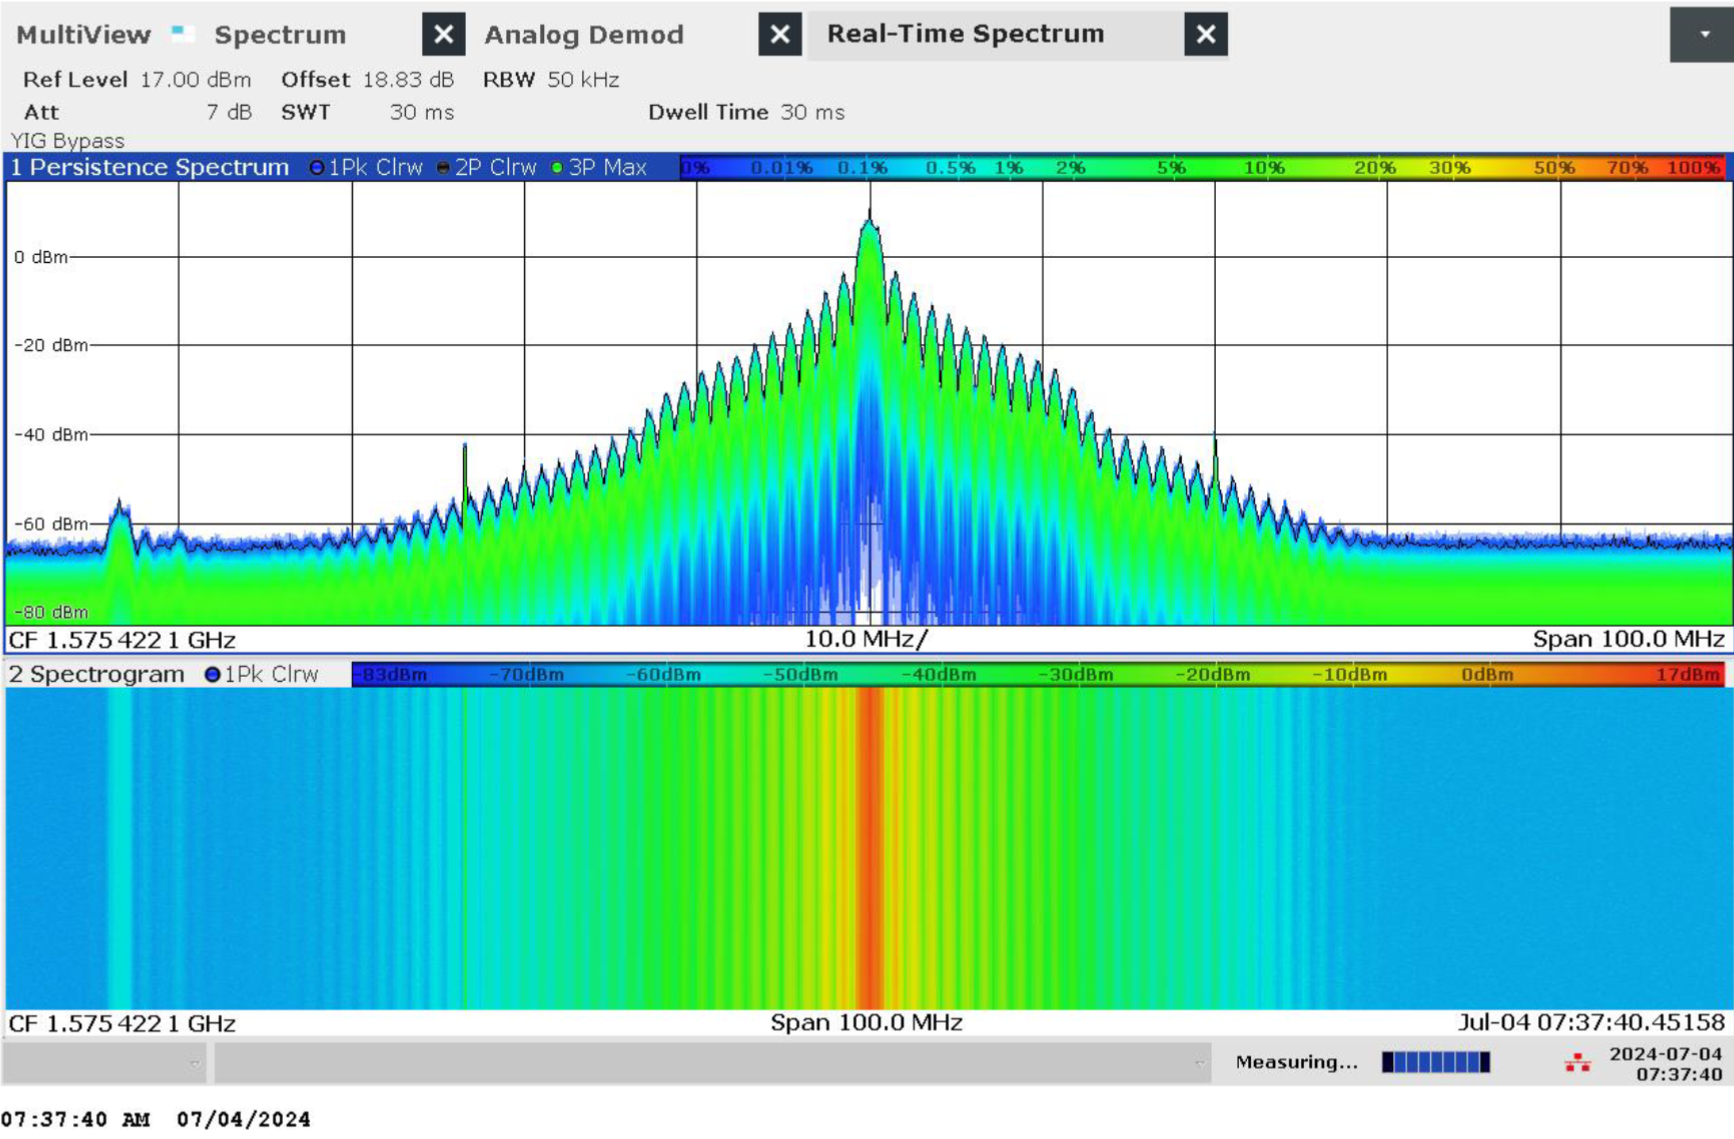
\includegraphics[width=\textwidth]{../graphics/appendixG/h1.1-6.png} 
\caption{Real-time persistence and spectrogram measurement with wider span of jammer H1.1 with antenna configuration L1 Narrow band High Power (NB HIGH PWR)}\end{figure}\begin{figure}[H]\includegraphics[width=\textwidth]{../graphics/appendixG/h1.1-7.png} 
\caption{Real-time persistence and spectrogram measurement of jammer H1.1 with antenna configuration L1 Wide band High Power (WB HIGH PWR)}\end{figure}\begin{figure}[H]\includegraphics[width=\textwidth]{../graphics/appendixG/h1.1-8.png} 
\caption{Real-time persistence and spectrogram measurement with wider span of jammer H1.1 with antenna configuration L1 Wide band High Power (WB HIGH PWR)}\end{figure}\begin{figure}[H]\includegraphics[width=\textwidth]{../graphics/appendixG/h1.1-9.png} 
\caption{Real-time persistence and spectrogram measurement with wider span of jammer H1.1 with antenna configuration L1 Continuous Wave band High Power (CW HIGH PWR)}\end{figure}\begin{figure}[H]\includegraphics[width=\textwidth]{../graphics/appendixG/h1.1-10.png} 
\caption{Real-time persistence and spectrogram measurement of jammer H1.1 with antenna configuration L1 Chirp High Power (CHIRP HIGH PWR)}\end{figure}\begin{figure}[H]\includegraphics[width=\textwidth]{../graphics/appendixG/h1.1-11.png} 
\caption{Time domain (analog demod) measurement of jammer H1.1 with antenna configuration L1 Narrow band High Power (NB HIGH PWR)}\end{figure}\begin{figure}[H]\includegraphics[width=\textwidth]{../graphics/appendixG/h1.1-12.png} 
\caption{Time domain (analog demod) measurement of jammer H1.1 with antenna configuration L1 Wide band High Power (WB HIGH PWR)}\end{figure}\begin{figure}[H]\includegraphics[width=\textwidth]{../graphics/appendixG/h1.1-13.png} 
\caption{Time domain (analog demod) measurement of jammer H1.1 with antenna configuration L1 Continuous Wave band High Power (CW HIGH PWR)}\end{figure}\begin{figure}[H]\includegraphics[width=\textwidth]{../graphics/appendixG/h1.1-14.png} 
\caption{Time domain (analog demod) measurement of jammer H1.1 with antenna configuration L1 Chirp High Power (CHIRP HIGH PWR)}\end{figure}\begin{figure}[H]\includegraphics[width=\textwidth]{../graphics/appendixG/h1.1-15.png} 
\caption{Frequency and power measurement of jammer H1.1 with antenna configuration L2 Narrow band High Power (NB HIGH PWR)}\end{figure}\begin{figure}[H]\includegraphics[width=\textwidth]{../graphics/appendixG/h1.1-16.png} 
\caption{Frequency and power measurement of jammer H1.1 with antenna configuration L2 Wide band High Power (WB HIGH PWR)}\end{figure}\begin{figure}[H]\includegraphics[width=\textwidth]{../graphics/appendixG/h1.1-17.png} 
\caption{Frequency and power measurement of jammer H1.1 with antenna configuration L2 Continuous Wave band High Power (CW HIGH PWR)}\end{figure}\begin{figure}[H]\includegraphics[width=\textwidth]{../graphics/appendixG/h1.1-18.png} 
\caption{Frequency and power measurement of jammer H1.1 with antenna configuration L2 Chirp High Power (CHIRP HIGH PWR)}\end{figure}\begin{figure}[H]\includegraphics[width=\textwidth]{../graphics/appendixG/h1.1-19.png} 
\caption{Real-time persistence and spectrogram measurement of jammer H1.1 with antenna configuration L2 Narrow band High Power (NB HIGH PWR)}\end{figure}\begin{figure}[H]\includegraphics[width=\textwidth]{../graphics/appendixG/h1.1-20.png} 
\caption{Real-time persistence and spectrogram measurement with wider span of jammer H1.1 with antenna configuration L2 Narrow band High Power (NB HIGH PWR)}\end{figure}\begin{figure}[H]\includegraphics[width=\textwidth]{../graphics/appendixG/h1.1-21.png} 
\caption{Real-time persistence and spectrogram measurement of jammer H1.1 with antenna configuration L2 Wide band High Power (WB HIGH PWR)}\end{figure}\begin{figure}[H]\includegraphics[width=\textwidth]{../graphics/appendixG/h1.1-22.png} 
\caption{Real-time persistence and spectrogram measurement with wider span of jammer H1.1 with antenna configuration L2 Wide band High Power (WB HIGH PWR)}\end{figure}\begin{figure}[H]\includegraphics[width=\textwidth]{../graphics/appendixG/h1.1-23.png} 
\caption{Real-time persistence and spectrogram measurement with wider span of jammer H1.1 with antenna configuration L2 Continuous Wave band High Power (CW HIGH PWR)}\end{figure}\begin{figure}[H]\includegraphics[width=\textwidth]{../graphics/appendixG/h1.1-24.png} 
\caption{Real-time persistence and spectrogram measurement of jammer H1.1 with antenna configuration L2 Chirp High Power (CHIRP HIGH PWR)}\end{figure}\begin{figure}[H]\includegraphics[width=\textwidth]{../graphics/appendixG/h1.1-25.png} 
\caption{Time domain (analog demod) measurement of jammer H1.1 with antenna configuration L2 Narrow band High Power (NB HIGH PWR)}\end{figure}\begin{figure}[H]\includegraphics[width=\textwidth]{../graphics/appendixG/h1.1-26.png} 
\caption{Time domain (analog demod) measurement of jammer H1.1 with antenna configuration L2 Wide band High Power (WB HIGH PWR)}\end{figure}\begin{figure}[H]\includegraphics[width=\textwidth]{../graphics/appendixG/h1.1-27.png} 
\caption{Time domain (analog demod) measurement of jammer H1.1 with antenna configuration L2 Continuous Wave band High Power (CW HIGH PWR)}\end{figure}\begin{figure}[H]\includegraphics[width=\textwidth]{../graphics/appendixG/h1.1-28.png} 
\caption{Time domain (analog demod) measurement of jammer H1.1 with antenna configuration L2 Chirp High Power (CHIRP HIGH PWR)}\end{figure}\subsection{Technical details on low-power jammer 'H1.2'}
\includegraphics[scale=0.4]{../graphics/appendixG/h1.2-photo.png}\\ \\ 
The jammer H1.2 belongs to the 'Handheld category' of jammers. It is a small and light battery driven jammer with an easy operation, just an on/off-button with a LED-light to indicate activation.\\H1.2 is an one-antenna, so-called 'L1-only', jammer, disrupting only the upper L-band.\\
\begin{table}[H]\centering
\begin{tabular}{|c|c|c|c|c|c|c|c|}\rowcolor[HTML]{C0C0C0} 
\hline
\makecell{Antenna} & \makecell{Centre frequency\\{[MHz]}} & \makecell{Bandwidth\\{[MHz]}} & \makecell{PSD\\{[dBm/MHz]}} & \makecell{TX total\\{[dBm]}} & \makecell{CF max\\{[dBm]}} & \makecell{Sweep rate\\{[µs]}} & \makecell{Modulation}\\ 
\hline
\makecell{L1} & \makecell{1575.22} & \makecell{21.99} & \makecell{14.35} & \makecell{27.78} & \makecell{9.36} & \makecell{6.08} & \makecell{Sawtooth}\\ 
\hline\end{tabular}\caption{Technical characteristics of H1.2 jammer}\label{table:tech_char_H1.2}\end{table}
\begin{figure}[H]\includegraphics[width=\textwidth]{../graphics/appendixG/h1.2-1.png} 
\caption{Frequency and power measurement of jammer H1.2}\end{figure}\begin{figure}[H]\includegraphics[width=\textwidth]{../graphics/appendixG/h1.2-2.png} 
\caption{Real-time persistence and spectrogram measurement of jammer H1.2}\end{figure}\begin{figure}[H]\includegraphics[width=\textwidth]{../graphics/appendixG/h1.2-3.png} 
\caption{Time domain (analog demod) measurement of jammer H1.2}\end{figure}\subsection{Technical details on low-power jammer 'H1.3'}
\includegraphics[scale=0.4]{../graphics/appendixG/h1.3-photo.png}\\ \\ 
H1.3 is a small, handheld and battery driven jammer using frequency hopping (normally commercially available jammers employ chirp signals, making this jammer an oddity).\\H1.3 is an one-antenna, so-called 'L1-only', jammer, disrupting only the upper L-band.\\\\Type of modulation: frequency hopping\\- Jumping between 6 separated frequencies. Every 50 ms the frequency increases 200 kHz, starting with 1574.62 MHz. After approximately 1 MHz the frequency jumps back to the start frequency at 1574.62 MHz.\\
\begin{table}[H]\centering
\begin{tabular}{|c|c|c|c|c|c|c|}\rowcolor[HTML]{C0C0C0} 
\hline
\makecell{Centre frequency\\{[MHz]}} & \makecell{Bandwidth\\{[MHz]}} & \makecell{PSD\\{[dBm/MHz]}} & \makecell{TX total\\{[dBm]}} & \makecell{CF max\\{[dBm]}} & \makecell{Sweep rate\\{[µs]}} & \makecell{Modulation}\\ 
\hline
\makecell{1575} & \makecell{1} & \makecell{N/A} & \makecell{N/A} & \makecell{N/A} & \makecell{5-8} & \makecell{Frequency hopping}\\ 
\hline\end{tabular}\caption{Technical characteristics of H1.3 jammer}\label{table:tech_char_H1.3}\end{table}
\begin{figure}[H]\includegraphics[width=\textwidth]{../graphics/appendixG/h1.3-1.png} 
\caption{Example measurement of H1.3 jammer}\end{figure}\subsection{Technical details on low-power jammer 'H1.4'}
Jammer H1.4 is assumed more or less identical to jammer H1.1 (originating from the same source and built by the same producer).\\
\subsection{Technical details on low-power jammer 'H1.5'}
Jammer H1.5 is assumed more or less identical to jammer H1.1 (originating from the same source and built by the same producer).\\
\subsection{Technical details on low-power jammer 'H2.1 and H2.2'}
\includegraphics[scale=0.4]{../graphics/appendixG/h2.1-photo.png}\\ \\ 
H2.1 and H2.2 are small and light handheld, battery driven jammers with built-in antennas.\\They are two-antenna, so-called 'L1+L2', jammers, disrupting both the upper and lower L-band.\\
\begin{table}[H]\centering
\begin{tabular}{|c|c|c|c|c|c|c|}\rowcolor[HTML]{C0C0C0} 
\hline
\makecell{Centre frequency\\{[MHz]}} & \makecell{Bandwidth\\{[MHz]}} & \makecell{PSD\\{[dBm/MHz]}} & \makecell{TX total\\{[dBm]}} & \makecell{CF max\\{[dBm]}} & \makecell{Sweep rate\\{[µs]}} & \makecell{Modulation}\\ 
\hline
\makecell{1580} & \makecell{20} & \makecell{N/A} & \makecell{N/A} & \makecell{N/A} & \makecell{9} & \makecell{Sawtooth}\\ 
\hline
\makecell{1227} & \makecell{20} & \makecell{N/A} & \makecell{N/A} & \makecell{N/A} & \makecell{9} & \makecell{Sawtooth}\\ 
\hline\end{tabular}\caption{Technical characteristics of H2.1-H2.2 jammer}\label{table:tech_char_H2.1-H2.2}\end{table}
\begin{figure}[H]\includegraphics[width=\textwidth]{../graphics/appendixG/h2.1-1.png} 
\caption{Example measurement of H2.1 and H2.2 jammer}\end{figure}\subsection{Technical details on low-power jammer 'H3.1'}
\includegraphics[scale=0.4]{../graphics/appendixG/h3.1-photo.png}\\ \\ 
The jammer H3.1 belongs to the 'Handheld category' of jammers. It is a small and light battery driven jammer with an easy operation, just an on/off-button with a LED-light to indicate activation.\\\\ H3.1 is a three-antenna, so-called 'multi-frequency', jammer, but not a 'multi-GNSS-jammer'. It jams three different bands, but only one channel is relevant for GNSS bands ('L1-only'), so disrupting only the upper L-band.\\\\Relevant GNSS antenna is marked: 'GPS'\\
\begin{table}[H]\centering
\begin{tabular}{|c|c|c|c|c|c|c|c|}\rowcolor[HTML]{C0C0C0} 
\hline
\makecell{Antenna} & \makecell{Centre frequency\\{[MHz]}} & \makecell{Bandwidth\\{[MHz]}} & \makecell{PSD\\{[dBm/MHz]}} & \makecell{TX total\\{[dBm]}} & \makecell{CF max\\{[dBm]}} & \makecell{Sweep rate\\{[µs]}} & \makecell{Modulation}\\ 
\hline
\makecell{'GPS'} & \makecell{1577.93} & \makecell{28.29} & \makecell{17.34} & \makecell{31.86} & \makecell{16.17} & \makecell{6.16} & \makecell{Sawtooth}\\ 
\hline\end{tabular}\caption{Technical characteristics of H3.1 jammer}\label{table:tech_char_H3.1}\end{table}
\begin{figure}[H]\includegraphics[width=\textwidth]{../graphics/appendixG/h3.1-1.png} 
\caption{Frequency and power measurement of jammer H3.1 on antenna 'GPS'}\end{figure}\begin{figure}[H]\includegraphics[width=\textwidth]{../graphics/appendixG/h3.1-2.png} 
\caption{Real-time persistence and spectrogram measurement of jammer H3.1 on antenna 'GPS'}\end{figure}\begin{figure}[H]\includegraphics[width=\textwidth]{../graphics/appendixG/h3.1-3.png} 
\caption{Time domain (analog demod) measurement of jammer H3.1 on antenna 'GPS'}\end{figure}\subsection{Technical details on low-power jammer 'H4.1'}
\includegraphics[scale=0.4]{../graphics/appendixG/h4.1-photo.png}\\ \\ 
The jammer H4.1 belongs to the 'Handheld category' of jammers. It is a small and relatively light battery driven jammer with a relatively easy operation, just an on/off-button with a LED-light to indicate activation and DIP switches to change between channels.\\\\H4.1 is a four-antenna, so-called 'L1+L2+L5+E6', jammer, disrupting both the upper and lower L-band.\\\\The four antennas are marked with numbers: '1' (L1), '2' (E6), '3' (L2) and '4' (L5)\\\\The jammer has additional noise (harmonics) in several other (non GNSS) frequency bands.\\
\begin{table}[H]\centering
\begin{tabular}{|c|c|c|c|c|c|c|c|}\rowcolor[HTML]{C0C0C0} 
\hline
\makecell{Antenna} & \makecell{Centre frequency\\{[MHz]}} & \makecell{Bandwidth\\{[MHz]}} & \makecell{PSD\\{[dBm/MHz]}} & \makecell{TX total\\{[dBm]}} & \makecell{CF max\\{[dBm]}} & \makecell{Sweep rate\\{[µs]}} & \makecell{Modulation}\\ 
\hline
\makecell{'1' (L1)} & \makecell{1548.02} & \makecell{102.67} & \makecell{21.14} & \makecell{41.25} & \makecell{25.20} & \makecell{8.82} & \makecell{Sawtooth}\\ 
\hline
\makecell{'2' (E6)} & \makecell{1261.92} & \makecell{48.80} & \makecell{22.38} & \makecell{39.26} & \makecell{22.33} & \makecell{8.86} & \makecell{Sawtooth}\\ 
\hline
\makecell{'3' (L2)} & \makecell{1220.34} & \makecell{47.88} & \makecell{21.08} & \makecell{37.88} & \makecell{20.29} & \makecell{8.82} & \makecell{Sawtooth}\\ 
\hline
\makecell{'4' (L5)} & \makecell{1182.32} & \makecell{39.66} & \makecell{22.87} & \makecell{38.85} & \makecell{22.83} & \makecell{8.84} & \makecell{Sawtooth}\\ 
\hline\end{tabular}\caption{Technical characteristics of H4.1 jammer}\label{table:tech_char_H4.1}\end{table}
\begin{figure}[H]\includegraphics[width=\textwidth]{../graphics/appendixG/h4.1-1.png} 
\caption{Frequency and power measurement of jammer H4.1 on antenna '1' (L1)}\end{figure}\begin{figure}[H]\includegraphics[width=\textwidth]{../graphics/appendixG/h4.1-2.png} 
\caption{Frequency and power measurement with wider span of jammer H4.1 on antenna '1' (L1)}\end{figure}\begin{figure}[H]\includegraphics[width=\textwidth]{../graphics/appendixG/h4.1-3.png} 
\caption{Frequency and power measurement of jammer H4.1 on antenna '2' (E6)}\end{figure}\begin{figure}[H]\includegraphics[width=\textwidth]{../graphics/appendixG/h4.1-4.png} 
\caption{Frequency and power measurement with wider span of jammer H4.1 on antenna '2' (E6)}\end{figure}\begin{figure}[H]\includegraphics[width=\textwidth]{../graphics/appendixG/h4.1-5.png} 
\caption{Frequency and power measurement of jammer H4.1 on antenna '3' (L2)}\end{figure}\begin{figure}[H]\includegraphics[width=\textwidth]{../graphics/appendixG/h4.1-6.png} 
\caption{Frequency and power measurement with wider span of jammer H4.1 on antenna '3' (L2)}\end{figure}\begin{figure}[H]\includegraphics[width=\textwidth]{../graphics/appendixG/h4.1-7.png} 
\caption{Frequency and power measurement of jammer H4.1 on antenna '4' (L5)}\end{figure}\begin{figure}[H]\includegraphics[width=\textwidth]{../graphics/appendixG/h4.1-8.png} 
\caption{Frequency and power measurement with wider span of jammer H4.1 on antenna '4' (L5)}\end{figure}\begin{figure}[H]\includegraphics[width=\textwidth]{../graphics/appendixG/h4.1-9.png} 
\caption{Real-time persistence and spectrogram measurement of jammer H4.1 on antenna '1' (L1)}\end{figure}\begin{figure}[H]\includegraphics[width=\textwidth]{../graphics/appendixG/h4.1-10.png} 
\caption{Real-time persistence and spectrogram measurement of jammer H4.1 on antenna '2' (E6)}\end{figure}\begin{figure}[H]\includegraphics[width=\textwidth]{../graphics/appendixG/h4.1-11.png} 
\caption{Real-time persistence and spectrogram measurement of jammer H4.1 on antenna '3' (L2)}\end{figure}\begin{figure}[H]\includegraphics[width=\textwidth]{../graphics/appendixG/h4.1-12.png} 
\caption{Real-time persistence and spectrogram measurement of jammer H4.1 on antenna '4' (L5)}\end{figure}\begin{figure}[H]\includegraphics[width=\textwidth]{../graphics/appendixG/h4.1-13.png} 
\caption{Time domain (analog demod) measurement of jammer H4.1 on antenna '1' (L1)}\end{figure}\begin{figure}[H]\includegraphics[width=\textwidth]{../graphics/appendixG/h4.1-14.png} 
\caption{Time domain (analog demod) measurement of jammer H4.1 on antenna '2' (E6)}\end{figure}\begin{figure}[H]\includegraphics[width=\textwidth]{../graphics/appendixG/h4.1-15.png} 
\caption{Time domain (analog demod) measurement of jammer H4.1 on antenna '3' (L2)}\end{figure}\begin{figure}[H]\includegraphics[width=\textwidth]{../graphics/appendixG/h4.1-16.png} 
\caption{Time domain (analog demod) measurement of jammer H4.1 on antenna '4' (L5)}\end{figure}\subsection{Technical details on low-power jammer 'H6.1'}
\includegraphics[scale=0.4]{../graphics/appendixG/h6.1-photo.png}\\ \\ 
The jammer H6.1 belongs to the 'Handheld category' of jammers. It is a larger but relatively light battery driven jammer with a relatively easy operation, just an on/off-button with a LED-light to indicate activation and DIP switches to change between channels.\\\\H6.1 is a six-antenna, so-called 'multi-frequency', jammer, but technically not a 'multi-GNSS-jammer'. It jams six different bands, but only two channels are relevant for GNSS bands, both in the upper L-band (so 'L1-only'), thus only disrupting the upper L-band.\\\\The most relevant GNSS antenna is marked '6'. The periphery antenna is marked '4'. To avoid disrupting non-GNSS services, use only antenna '6'.\\
\begin{table}[H]\centering
\begin{tabular}{|c|c|c|c|c|c|c|c|}\rowcolor[HTML]{C0C0C0} 
\hline
\makecell{Antenna} & \makecell{Centre frequency\\{[MHz]}} & \makecell{Bandwidth\\{[MHz]}} & \makecell{PSD\\{[dBm/MHz]}} & \makecell{TX total\\{[dBm]}} & \makecell{CF max\\{[dBm]}} & \makecell{Sweep rate\\{[µs]}} & \makecell{Modulation}\\ 
\hline
\makecell{'4'} & \makecell{1621.23} & \makecell{87.50} & \makecell{2.89} & \makecell{22.31} & \makecell{5.57} & \makecell{5.9} & \makecell{Sawtooth}\\ 
\hline
\makecell{'6' (L1)} & \makecell{1581.18} & \makecell{22.24} & \makecell{24.60} & \makecell{38.07} & \makecell{24.37} & \makecell{5.86} & \makecell{Sawtooth}\\ 
\hline\end{tabular}\caption{Technical characteristics of H6.1 jammer}\label{table:tech_char_H6.1}\end{table}
\begin{figure}[H]\includegraphics[width=\textwidth]{../graphics/appendixG/h6.1-1.png} 
\caption{Frequency and power measurement of jammer H6.1 on antenna '6' (L1)}\end{figure}\begin{figure}[H]\includegraphics[width=\textwidth]{../graphics/appendixG/h6.1-2.png} 
\caption{Frequency and power measurement of jammer H6.1 on antenna '4'}\end{figure}\begin{figure}[H]\includegraphics[width=\textwidth]{../graphics/appendixG/h6.1-3.png} 
\caption{Real-time persistence and spectrogram measurement of jammer H6.1 on antenna '6' (L1)}\end{figure}\begin{figure}[H]\includegraphics[width=\textwidth]{../graphics/appendixG/h6.1-4.png} 
\caption{Real-time persistence and spectrogram measurement of jammer H6.1 on antenna '4'}\end{figure}\begin{figure}[H]\includegraphics[width=\textwidth]{../graphics/appendixG/h6.1-5.png} 
\caption{Time domain (analog demod) measurement of jammer H6.1 on antenna '6' (L1)}\end{figure}\begin{figure}[H]\includegraphics[width=\textwidth]{../graphics/appendixG/h6.1-6.png} 
\caption{Time domain (analog demod) measurement of jammer H6.1 on antenna '4'}\end{figure}\subsection{Technical details on low-power jammer 'H6.2'}
\includegraphics[scale=0.4]{../graphics/appendixG/h6.1-photo.png}\\ \\ 
The jammer H6.2 belongs to the 'Handheld category' of jammers. It is a larger but relatively light battery driven jammer with a relatively easy  peration, just an on/off-button with a LED-light to indicate activation and DIP switches to change between channels.\\\\ H6.2 is a six-antenna, so-called  multi-frequency', jammer. It jams six different bands, but only three channels are relevant for GNSS bands ('L1+L2+L5'), thus disrupting the upper and lower L-band.\\\\The relevant antennas are marked with numbers: '4' (L1), '5' (L5) and '6' (L2). The jammer has additional noise in several other (non  GNSS) frequency bands, but with significant lower power.\\
\begin{table}[H]\centering
\begin{tabular}{|c|c|c|c|c|c|c|c|}\rowcolor[HTML]{C0C0C0} 
\hline
\makecell{Antenna} & \makecell{Centre frequency\\{[MHz]}} & \makecell{Bandwidth\\{[MHz]}} & \makecell{PSD\\{[dBm/MHz]}} & \makecell{TX total\\{[dBm]}} & \makecell{CF max\\{[dBm]}} & \makecell{Sweep rate\\{[µs]}} & \makecell{Modulation}\\ 
\hline
\makecell{'4' (L1)} & \makecell{1581.51} & \makecell{30.00} & \makecell{26.50} & \makecell{41.27} & \makecell{25.99} & \makecell{7.0/28.2} & \makecell{Sawtooth modulated unto sinus}\\ 
\hline
\makecell{'5' (L5)} & \makecell{1154.62} & \makecell{110.77} & \makecell{19.98} & \makecell{40.42} & \makecell{24.57} & \makecell{7.14} & \makecell{Sawtooth}\\ 
\hline
\makecell{'6' (L2)} & \makecell{1247.94} & \makecell{113.14} & \makecell{21.85} & \makecell{42.39} & \makecell{26.78} & \makecell{7.1} & \makecell{Sawtooth}\\ 
\hline\end{tabular}\caption{Technical characteristics of H6.2 jammer}\label{table:tech_char_H6.2}\end{table}
\begin{figure}[H]\includegraphics[width=\textwidth]{../graphics/appendixG/h6.2-1.png} 
\caption{Frequency and power measurement of jammer H6.2 on antenna '4' (L1)}\end{figure}\begin{figure}[H]\includegraphics[width=\textwidth]{../graphics/appendixG/h6.2-2.png} 
\caption{Frequency and power measurement with wider band of jammer H6.2 on antenna '4' (L1)}\end{figure}\begin{figure}[H]\includegraphics[width=\textwidth]{../graphics/appendixG/h6.2-3.png} 
\caption{Frequency and power measurement of jammer H6.2 on antenna '5' (L5)}\end{figure}\begin{figure}[H]\includegraphics[width=\textwidth]{../graphics/appendixG/h6.2-4.png} 
\caption{Frequency and power measurement of jammer H6.2 on antenna '6' (L2)}\end{figure}\begin{figure}[H]\includegraphics[width=\textwidth]{../graphics/appendixG/h6.2-5.png} 
\caption{Real-time persistence and spectrogram measurement of jammer H6.2 on antenna '4' (L1)}\end{figure}\begin{figure}[H]\includegraphics[width=\textwidth]{../graphics/appendixG/h6.2-6.png} 
\caption{Real-time persistence and spectrogram measurement with wider span of jammer H6.2 on antenna '4' (L1)}\end{figure}\begin{figure}[H]\includegraphics[width=\textwidth]{../graphics/appendixG/h6.2-7.png} 
\caption{Real-time persistence and spectrogram measurement of jammer H6.2 on antenna '5' (L5)}\end{figure}\begin{figure}[H]\includegraphics[width=\textwidth]{../graphics/appendixG/h6.2-8.png} 
\caption{Real-time persistence and spectrogram measurement of jammer H6.2 on antenna '6' (L2)}\end{figure}\begin{figure}[H]\includegraphics[width=\textwidth]{../graphics/appendixG/h6.2-9.png} 
\caption{Time domain (analog demod) measurement with wider sweep of jammer H6.2 on antenna '4' (L1)}\end{figure}\begin{figure}[H]\includegraphics[width=\textwidth]{../graphics/appendixG/h6.2-10.png} 
\caption{Time domain (analog demod) measurement of jammer H6.2 on antenna '5' (L5)}\end{figure}\begin{figure}[H]\includegraphics[width=\textwidth]{../graphics/appendixG/h6.2-11.png} 
\caption{Time domain (analog demod) measurement of jammer H6.2 on antenna '6' (L2)}\end{figure}\subsection{Technical details on low-power jammer 'H6.3'}
\includegraphics[scale=0.4]{../graphics/appendixG/h6.1-photo.png}\\ \\ 
The jammer H6.3 belongs to the 'Handheld category' of jammers. It is a larger but relatively light battery driven jammer with a relatively easy  peration, just an on/off-button with a LED-light to indicate activation and DIP switches to change between channels.\\\\ H6.2 is a six-antenna, so-called  multi-frequency', jammer. It jams six different bands, but only three channels are relevant for GNSS bands ('L1+L2+L5'), thus disrupting the upper and lower L-band.\\\\The relevant antennas are marked with numbers: '4' (L1), '5' (L5) and '6' (L2).\\
\begin{table}[H]\centering
\begin{tabular}{|c|c|c|c|c|c|c|c|}\rowcolor[HTML]{C0C0C0} 
\hline
\makecell{Antenna} & \makecell{Centre frequency\\{[MHz]}} & \makecell{Bandwidth\\{[MHz]}} & \makecell{PSD\\{[dBm/MHz]}} & \makecell{TX total\\{[dBm]}} & \makecell{CF max\\{[dBm]}} & \makecell{Sweep rate\\{[µs]}} & \makecell{Modulation}\\ 
\hline
\makecell{'4' (L1)} & \makecell{1581.37} & \makecell{26.50} & \makecell{25.54} & \makecell{39.77} & \makecell{25.46} & \makecell{7.1} & \makecell{Sawtooth}\\ 
\hline
\makecell{'5' (L5)} & \makecell{1152.73} & \makecell{112.05} & \makecell{19.50} & \makecell{39.99} & \makecell{24.36} & \makecell{7.06} & \makecell{Sawtooth}\\ 
\hline
\makecell{'6' (L2)} & \makecell{1248.65} & \makecell{111.06} & \makecell{21.80} & \makecell{42.25} & \makecell{26.65} & \makecell{7.08} & \makecell{Sawtooth}\\ 
\hline\end{tabular}\caption{Technical characteristics of H6.3 jammer}\label{table:tech_char_H6.3}\end{table}
\begin{figure}[H]\includegraphics[width=\textwidth]{../graphics/appendixG/h6.3-1.png} 
\caption{Frequency and power measurement of jammer H6.3 on antenna '4' (L1)}\end{figure}\begin{figure}[H]\includegraphics[width=\textwidth]{../graphics/appendixG/h6.3-2.png} 
\caption{Frequency and power measurement of jammer H6.3 on antenna '5' (L5)}\end{figure}\begin{figure}[H]\includegraphics[width=\textwidth]{../graphics/appendixG/h6.3-3.png} 
\caption{Frequency and power measurement of jammer H6.3 on antenna '6' (L2)}\end{figure}\begin{figure}[H]\includegraphics[width=\textwidth]{../graphics/appendixG/h6.3-4.png} 
\caption{Real-time persistence and spectrogram measurement of jammer H6.3 on antenna '4' (L1)}\end{figure}\begin{figure}[H]\includegraphics[width=\textwidth]{../graphics/appendixG/h6.3-5.png} 
\caption{Real-time persistence and spectrogram measurement with wider span of jammer H6.3 on antenna '4' (L1)}\end{figure}\begin{figure}[H]\includegraphics[width=\textwidth]{../graphics/appendixG/h6.3-6.png} 
\caption{Real-time persistence and spectrogram measurement of jammer H6.3 on antenna '5' (L5)}\end{figure}\begin{figure}[H]\includegraphics[width=\textwidth]{../graphics/appendixG/h6.3-7.png} 
\caption{Real-time persistence and spectrogram measurement of jammer H6.3 on antenna '6' (L2)}\end{figure}\begin{figure}[H]\includegraphics[width=\textwidth]{../graphics/appendixG/h6.3-8.png} 
\caption{Time domain (analog demod) measurement of jammer H6.3 on antenna '4' (L1)}\end{figure}\begin{figure}[H]\includegraphics[width=\textwidth]{../graphics/appendixG/h6.3-9.png} 
\caption{Time domain (analog demod) measurement with wider sweep of jammer H6.3 on antenna '4' (L1)}\end{figure}\begin{figure}[H]\includegraphics[width=\textwidth]{../graphics/appendixG/h6.3-10.png} 
\caption{Time domain (analog demod) measurement of jammer H6.3 on antenna '5' (L5)}\end{figure}\begin{figure}[H]\includegraphics[width=\textwidth]{../graphics/appendixG/h6.3-11.png} 
\caption{Time domain (analog demod) measurement of jammer H6.3 on antenna '6' (L2)}\end{figure}\subsection{Technical details on low-power jammer 'H6.4'}
\includegraphics[scale=0.4]{../graphics/appendixG/h6.4-photo.png}\\ \\ 
The jammer H6.4 belongs to the 'Handheld category' of jammers. It is a larger but relatively light battery driven jammer with a relatively easy  peration, just an on/off-button with a LED-light to indicate activation and DIP switches to change between channels.\\\\ H6.4 is a six-antenna, so-called  multi-frequency', jammer. It jams six different bands, but only three channels are relevant for GNSS bands ('L1+L2+L5'), thus disrupting the upper and lower L-band.\\\\The relevant antennas are marked with numbers: '1' (L5), '3' (L2) and '5' (L1).\\
\begin{table}[H]\centering
\begin{tabular}{|c|c|c|c|c|c|c|c|}\rowcolor[HTML]{C0C0C0} 
\hline
\makecell{Antenna} & \makecell{Centre frequency\\{[MHz]}} & \makecell{Bandwidth\\{[MHz]}} & \makecell{PSD\\{[dBm/MHz]}} & \makecell{TX total\\{[dBm]}} & \makecell{CF max\\{[dBm]}} & \makecell{Sweep rate\\{[µs]}} & \makecell{Modulation}\\ 
\hline
\makecell{'1' (L5)} & \makecell{1176.66} & \makecell{17.23} & \makecell{16.54} & \makecell{28.91} & \makecell{19.30} & \makecell{10.62} & \makecell{Triangle}\\ 
\hline
\makecell{'3' (L2)} & \makecell{1248.01} & \makecell{85.41} & \makecell{23.54} & \makecell{42.86} & \makecell{26.15} & \makecell{10.3} & \makecell{Triangle}\\ 
\hline
\makecell{'5' (L1)} & \makecell{1593.36} & \makecell{81.28} & \makecell{22.82} & \makecell{41.92} & \makecell{25.63} & \makecell{11} & \makecell{Triangle}\\ 
\hline\end{tabular}\caption{Technical characteristics of H6.4 jammer}\label{table:tech_char_H6.4}\end{table}
\begin{figure}[H]\includegraphics[width=\textwidth]{../graphics/appendixG/h6.4-1.png} 
\caption{Frequency and power measurement of jammer H6.4 on antenna '1' (L5)}\end{figure}\begin{figure}[H]\includegraphics[width=\textwidth]{../graphics/appendixG/h6.4-2.png} 
\caption{Frequency and power measurement of jammer H6.4 on antenna '3' (L2)}\end{figure}\begin{figure}[H]\includegraphics[width=\textwidth]{../graphics/appendixG/h6.4-3.png} 
\caption{Frequency and power measurement of jammer H6.4 on antenna '5' (L1)}\end{figure}\begin{figure}[H]\includegraphics[width=\textwidth]{../graphics/appendixG/h6.4-4.png} 
\caption{Real-time persistence and spectrogram measurement of jammer H6.4 on antenna '1' (L5)}\end{figure}\begin{figure}[H]\includegraphics[width=\textwidth]{../graphics/appendixG/h6.4-5.png} 
\caption{Real-time persistence and spectrogram measurement of jammer H6.4 on antenna '3' (L2)}\end{figure}\begin{figure}[H]\includegraphics[width=\textwidth]{../graphics/appendixG/h6.4-6.png} 
\caption{Real-time persistence and spectrogram measurement of jammer H6.4 on antenna '5' (L1)}\end{figure}\begin{figure}[H]\includegraphics[width=\textwidth]{../graphics/appendixG/h6.4-7.png} 
\caption{Time domain (analog demod) measurement of jammer H6.4 on antenna '1' (L5)}\end{figure}\begin{figure}[H]\includegraphics[width=\textwidth]{../graphics/appendixG/h6.4-8.png} 
\caption{Time domain (analog demod) measurement of jammer H6.4 on antenna '3' (L2)}\end{figure}\begin{figure}[H]\includegraphics[width=\textwidth]{../graphics/appendixG/h6.4-9.png} 
\caption{Time domain (analog demod) measurement of jammer H6.4 on antenna '5' (L1)}\end{figure}\subsection{Technical details on low-power jammer 'H6.5'}
\includegraphics[scale=0.4]{../graphics/appendixG/h6.4-photo.png}\\ \\ 
The jammer H6.5 belongs to the 'Handheld category' of jammers. It is a larger but relatively light battery driven jammer with a relatively easy  peration, just an on/off-button with a LED-light to indicate activation and DIP switches to change between channels.\\\\ H6.5 is a six-antenna, so-called  multi-frequency', jammer. It jams six different bands, but only three channels are relevant for GNSS bands ('L1+L2+L5'), thus disrupting the upper and lower L-band.\\\\The relevant antennas are marked with numbers: '1' (L5), '3' (L2) and '5' (L1).\\
\begin{table}[H]\centering
\begin{tabular}{|c|c|c|c|c|c|c|c|}\rowcolor[HTML]{C0C0C0} 
\hline
\makecell{Antenna} & \makecell{Centre frequency\\{[MHz]}} & \makecell{Bandwidth\\{[MHz]}} & \makecell{PSD\\{[dBm/MHz]}} & \makecell{TX total\\{[dBm]}} & \makecell{CF max\\{[dBm]}} & \makecell{Sweep rate\\{[µs]}} & \makecell{Modulation}\\ 
\hline
\makecell{'1' (L5)} & \makecell{1180.33} & \makecell{24.28} & \makecell{24.73} & \makecell{38.58} & \makecell{27.66} & \makecell{10.26} & \makecell{Triangle}\\ 
\hline
\makecell{'3' (L2)} & \makecell{1247.05} & \makecell{82.22} & \makecell{23.22} & \makecell{42.37} & \makecell{25.77} & \makecell{10.32} & \makecell{Triangle}\\ 
\hline
\makecell{'5' (L1)} & \makecell{1595.60} & \makecell{80.12} & \makecell{22.62} & \makecell{41.65} & \makecell{25.41} & \makecell{10.30} & \makecell{Triangle}\\ 
\hline\end{tabular}\caption{Technical characteristics of H6.5 jammer}\label{table:tech_char_H6.5}\end{table}
\begin{figure}[H]\includegraphics[width=\textwidth]{../graphics/appendixG/h6.5-1.png} 
\caption{Frequency and power measurement of jammer H6.5 on antenna '1' (L5)}\end{figure}\begin{figure}[H]\includegraphics[width=\textwidth]{../graphics/appendixG/h6.5-2.png} 
\caption{Frequency and power measurement of jammer H6.5 on antenna '3' (L2)}\end{figure}\begin{figure}[H]\includegraphics[width=\textwidth]{../graphics/appendixG/h6.5-3.png} 
\caption{Frequency and power measurement of jammer H6.5 on antenna '5' (L1)}\end{figure}\begin{figure}[H]\includegraphics[width=\textwidth]{../graphics/appendixG/h6.5-4.png} 
\caption{Real-time persistence and spectrogram measurement of jammer H6.5 on antenna '1' (L5)}\end{figure}\begin{figure}[H]\includegraphics[width=\textwidth]{../graphics/appendixG/h6.5-5.png} 
\caption{Real-time persistence and spectrogram measurement of jammer H6.5 on antenna '3' (L2)}\end{figure}\begin{figure}[H]\includegraphics[width=\textwidth]{../graphics/appendixG/h6.5-6.png} 
\caption{Real-time persistence and spectrogram measurement of jammer H6.5 on antenna '5' (L1)}\end{figure}\begin{figure}[H]\includegraphics[width=\textwidth]{../graphics/appendixG/h6.5-7.png} 
\caption{Time domain (analog demod) measurement of jammer H6.5 on antenna '1' (L5)}\end{figure}\begin{figure}[H]\includegraphics[width=\textwidth]{../graphics/appendixG/h6.5-8.png} 
\caption{Time domain (analog demod) measurement of jammer H6.5 on antenna '3' (L2)}\end{figure}\begin{figure}[H]\includegraphics[width=\textwidth]{../graphics/appendixG/h6.5-9.png} 
\caption{Time domain (analog demod) measurement of jammer H6.5 on antenna '5' (L1)}\end{figure}\subsection{Technical details on low-power jammer 'H6.6'}
\includegraphics[scale=0.4]{../graphics/appendixG/h6.4-photo.png}\\ \\ 
The jammer H6.6 belongs to the 'Handheld category' of jammers. It is a larger but relatively light battery driven jammer with a relatively easy  peration, just an on/off-button with a LED-light to indicate activation and DIP switches to change between channels.\\\\ H6.6 is a six-antenna, so-called  multi-frequency', jammer. It jams six different bands, but only three channels are relevant for GNSS bands ('L1+L2+L5'), thus disrupting the upper and lower L-band.\\\\The relevant antennas are marked with numbers: '1' (L5), '3' (L2) and '5' (L1).\\
\begin{table}[H]\centering
\begin{tabular}{|c|c|c|c|c|c|c|c|}\rowcolor[HTML]{C0C0C0} 
\hline
\makecell{Antenna} & \makecell{Centre frequency\\{[MHz]}} & \makecell{Bandwidth\\{[MHz]}} & \makecell{PSD\\{[dBm/MHz]}} & \makecell{TX total\\{[dBm]}} & \makecell{CF max\\{[dBm]}} & \makecell{Sweep rate\\{[µs]}} & \makecell{Modulation}\\ 
\hline
\makecell{'1' (L5)} & \makecell{1178.53} & \makecell{21.01} & \makecell{24.93} & \makecell{38.15} & \makecell{27.94} & \makecell{10.00} & \makecell{Triangle}\\ 
\hline
\makecell{'3' (L2)} & \makecell{1247.30} & \makecell{88.06} & \makecell{23.65} & \makecell{43.10} & \makecell{26.28} & \makecell{9.92} & \makecell{Triangle}\\ 
\hline
\makecell{'5' (L1)} & \makecell{1592.48} & \makecell{73.60} & \makecell{22.84} & \makecell{41.51} & \makecell{25.60} & \makecell{10.46} & \makecell{Triangle}\\ 
\hline\end{tabular}\caption{Technical characteristics of H6.6 jammer}\label{table:tech_char_H6.6}\end{table}
\begin{figure}[H]\includegraphics[width=\textwidth]{../graphics/appendixG/h6.6-1.png} 
\caption{Frequency and power measurement of jammer H6.6 on antenna '1' (L5)}\end{figure}\begin{figure}[H]\includegraphics[width=\textwidth]{../graphics/appendixG/h6.6-2.png} 
\caption{Frequency and power measurement of jammer H6.6 on antenna '3' (L2)}\end{figure}\begin{figure}[H]\includegraphics[width=\textwidth]{../graphics/appendixG/h6.6-3.png} 
\caption{Frequency and power measurement of jammer H6.6 on antenna '5' (L1)}\end{figure}\begin{figure}[H]\includegraphics[width=\textwidth]{../graphics/appendixG/h6.6-4.png} 
\caption{Real-time persistence and spectrogram measurement of jammer H6.6 on antenna '1' (L5)}\end{figure}\begin{figure}[H]\includegraphics[width=\textwidth]{../graphics/appendixG/h6.6-5.png} 
\caption{Real-time persistence and spectrogram measurement of jammer H6.6 on antenna '3' (L2)}\end{figure}\begin{figure}[H]\includegraphics[width=\textwidth]{../graphics/appendixG/h6.6-6.png} 
\caption{Real-time persistence and spectrogram measurement of jammer H6.6 on antenna '5' (L1)}\end{figure}\begin{figure}[H]\includegraphics[width=\textwidth]{../graphics/appendixG/h6.6-7.png} 
\caption{Time domain (analog demod) measurement of jammer H6.6 on antenna '1' (L5)}\end{figure}\begin{figure}[H]\includegraphics[width=\textwidth]{../graphics/appendixG/h6.6-8.png} 
\caption{Time domain (analog demod) measurement of jammer H6.6 on antenna '3' (L2)}\end{figure}\begin{figure}[H]\includegraphics[width=\textwidth]{../graphics/appendixG/h6.6-9.png} 
\caption{Time domain (analog demod) measurement of jammer H6.6 on antenna '5' (L1)}\end{figure}\subsection{Technical details on low-power jammer 'F6.1'}
\includegraphics[scale=0.4]{../graphics/appendixG/f6.1-photo.png}\\ \\ 
The jammer F6.1 belongs to the 'Permanently installed (Fixed)' of jammers. It is a large and heavy tabletop type of jammer, in need of constant power supply with a relatively easy operation, just an on/off-button with a LED-light to indicate activation and DIP switches to change between channels.\\\\F6.1 is a six-antenna, so-called 'multi-frequency', jammer. It jams six different bands, but only four channels are relevant for GNSS bands ('L1+L2+L5'), thus disrupting the upper and lower L-band.\\\\The relevant antennas are marked with letters and numbers: 'F2' (L1), 'F3' (L1), 'F4' (L2) and 'F6' (L5)\\\\This jammer has the possibility to adjust the output power, with a power control knob for each antenna. The measurements below are all done at maximum power.\\
\begin{table}[H]\centering
\begin{tabular}{|c|c|c|c|c|c|c|c|}\rowcolor[HTML]{C0C0C0} 
\hline
\makecell{Antenna} & \makecell{Centre frequency\\{[MHz]}} & \makecell{Bandwidth\\{[MHz]}} & \makecell{PSD\\{[dBm/MHz]}} & \makecell{TX total\\{[dBm]}} & \makecell{CF max\\{[dBm]}} & \makecell{Sweep rate\\{[µs]}} & \makecell{Modulation}\\ 
\hline
\makecell{'F2' (L1)} & \makecell{1592.59} & \makecell{66.55} & \makecell{31.49} & \makecell{49.72} & \makecell{34.85} & \makecell{6.46/98.50} & \makecell{sinus / FM-modulert}\\ 
\hline
\makecell{'F3' (L1)} & \makecell{1589.40} & \makecell{73.75} & \makecell{27.45} & \makecell{46.13} & \makecell{29.14} & \makecell{6.24} & \makecell{sinus}\\ 
\hline
\makecell{'F4' (L2)} & \makecell{1243.65} & \makecell{76.22} & \makecell{25.42} & \makecell{44.24} & \makecell{26.94} & \makecell{6.20/155.00} & \makecell{sinus / FM-modulert}\\ 
\hline
\makecell{'F6' (L5)} & \makecell{1177.93} & \makecell{16.58} & \makecell{24.93} & \makecell{37.13} & \makecell{18.51} & \makecell{5.96} & \makecell{sinus}\\ 
\hline\end{tabular}\caption{Technical characteristics of F6.1 jammer}\label{table:tech_char_F6.1}\end{table}
\begin{figure}[H]\includegraphics[width=\textwidth]{../graphics/appendixG/f6.1-1.png} 
\caption{Frequency and power measurement of jammer F6.1 on antenna 'F2' (L1)}\end{figure}\begin{figure}[H]\includegraphics[width=\textwidth]{../graphics/appendixG/f6.1-2.png} 
\caption{Frequency and power measurement of jammer F6.1 on antenna 'F3' (L1)}\end{figure}\begin{figure}[H]\includegraphics[width=\textwidth]{../graphics/appendixG/f6.1-3.png} 
\caption{Frequency and power measurement of jammer F6.1 on antenna 'F4' (L2)}\end{figure}\begin{figure}[H]\includegraphics[width=\textwidth]{../graphics/appendixG/f6.1-4.png} 
\caption{Frequency and power measurement of jammer F6.1 on antenna 'F6' (L5)}\end{figure}\begin{figure}[H]\includegraphics[width=\textwidth]{../graphics/appendixG/f6.1-5.png} 
\caption{Real-time persistence and spectrogram measurement of jammer F6.1 on antenna 'F2' (L1)}\end{figure}\begin{figure}[H]\includegraphics[width=\textwidth]{../graphics/appendixG/f6.1-6.png} 
\caption{Real-time persistence and spectrogram measurement of jammer F6.1 on antenna 'F3' (L1)}\end{figure}\begin{figure}[H]\includegraphics[width=\textwidth]{../graphics/appendixG/f6.1-7.png} 
\caption{Real-time persistence and spectrogram measurement of jammer F6.1 on antenna 'F4' (L2)}\end{figure}\begin{figure}[H]\includegraphics[width=\textwidth]{../graphics/appendixG/f6.1-8.png} 
\caption{Real-time persistence and spectrogram measurement of jammer F6.1 on antenna 'F6' (L5)}\end{figure}\begin{figure}[H]\includegraphics[width=\textwidth]{../graphics/appendixG/f6.1-9.png} 
\caption{Time domain (analog demod) measurement of jammer F6.1 on antenna 'F2' (L1)}\end{figure}\begin{figure}[H]\includegraphics[width=\textwidth]{../graphics/appendixG/f6.1-10.png} 
\caption{Time domain (analog demod) measurement with wider span of jammer F6.1 on antenna 'F2' (L1)}\end{figure}\begin{figure}[H]\includegraphics[width=\textwidth]{../graphics/appendixG/f6.1-11.png} 
\caption{Time domain (analog demod) measurement of jammer F6.1 on antenna 'F3' (L1)}\end{figure}\begin{figure}[H]\includegraphics[width=\textwidth]{../graphics/appendixG/f6.1-12.png} 
\caption{Time domain (analog demod) measurement with wider span of jammer F6.1 on antenna 'F3' (L1)}\end{figure}\begin{figure}[H]\includegraphics[width=\textwidth]{../graphics/appendixG/f6.1-13.png} 
\caption{Time domain (analog demod) measurement of jammer F6.1 on antenna 'F4' (L2)}\end{figure}\begin{figure}[H]\includegraphics[width=\textwidth]{../graphics/appendixG/f6.1-14.png} 
\caption{Time domain (analog demod) measurement with wider span of jammer F6.1 on antenna 'F4' (L2)}\end{figure}\begin{figure}[H]\includegraphics[width=\textwidth]{../graphics/appendixG/f6.1-15.png} 
\caption{Time domain (analog demod) measurement of jammer F6.1 on antenna 'F6' (L5)}\end{figure}\begin{figure}[H]\includegraphics[width=\textwidth]{../graphics/appendixG/f6.1-16.png} 
\caption{Time domain (analog demod) measurement with wider span of jammer F6.1 on antenna 'F6' (L5)}\end{figure}\subsection{Technical details on low-power jammer 'H8.1'}
\includegraphics[scale=0.4]{../graphics/appendixG/h8.1-photo.png}\\ \\ 
The jammer H8.1 belongs to the 'Handheld category' of jammers. It is a larger but relatively light battery driven jammer with a relatively easy operation, just an on/off-button with a LED-light to indicate activation and DIP switches to change between channels.\\\\H8.1 is a eight-antenna, so-called 'multi-frequency', jammer, but not a 'multi-GNSS-jammer'. It jams eight different bands, but only one GNSS-band ('L1-only'), so disrupting only the upper L-band.\\\\Relevant GNSS antenna is marked: '6'\\
\begin{table}[H]\centering
\begin{tabular}{|c|c|c|c|c|c|c|c|}\rowcolor[HTML]{C0C0C0} 
\hline
\makecell{Antenna} & \makecell{Centre frequency\\{[MHz]}} & \makecell{Bandwidth\\{[MHz]}} & \makecell{PSD\\{[dBm/MHz]}} & \makecell{TX total\\{[dBm]}} & \makecell{CF max\\{[dBm]}} & \makecell{Sweep rate\\{[µs]}} & \makecell{Modulation}\\ 
\hline
\makecell{'6'} & \makecell{1593.30} & \makecell{77.14} & \makecell{23.48} & \makecell{42.35} & \makecell{26.59} & \makecell{10.47} & \makecell{Triangle}\\ 
\hline\end{tabular}\caption{Technical characteristics of H8.1 jammer}\label{table:tech_char_H8.1}\end{table}
\begin{figure}[H]\includegraphics[width=\textwidth]{../graphics/appendixG/h8.1-1.png} 
\caption{Frequency and power measurement of jammer H8.1 on antenna '6'}\end{figure}\begin{figure}[H]\includegraphics[width=\textwidth]{../graphics/appendixG/h8.1-2.png} 
\caption{Real-time persistence and spectrogram measurement of jammer H8.1 on antenna '6'}\end{figure}\begin{figure}[H]\includegraphics[width=\textwidth]{../graphics/appendixG/h8.1-1.png} 
\caption{Time domain (analog demod) measurement of jammer H8.1 on antenna '6'}\end{figure}